\documentclass[mathpazo]{cicp}
\usepackage{times,amsmath,amsbsy,amssymb,amscd,mathrsfs}
%\usepackage{slashbox}\usepackage{graphicx,subfigure,epstopdf,wrapfig,chemarrow}

\usepackage{algorithm2e} 
\usepackage{multicol,multirow}
\usepackage{mathtools}
\usepackage[usenames,dvipsnames,svgnames,table]{xcolor}
\usepackage[all]{xy}
\usepackage{wrapfig}
\usepackage{tcolorbox}
\usepackage{booktabs} 

\usepackage[labelformat=empty]{subfig}
%\usepackage[hang,small,bf]{caption}

\usepackage{tikz,tikz-cd}
\usepackage[utf8]{inputenc}
\usepackage{pgfplots} 
\usepackage{pgfgantt}
\usepackage{pdflscape}
\pgfplotsset{compat=newest} 
\pgfplotsset{plot coordinates/math parser=false}
\newlength\fwidth

%\usepackage[notcite,notref]{showkeys}
\usepackage[numbered]{mcode}

\definecolor{myBlue}{rgb}{0.0,0.0,0.55}
%\definecolor{green}{rgb}{0.0,0.7,0.2}
\usepackage[pdftex,colorlinks=true,citecolor=myBlue,linkcolor=myBlue]{hyperref}

\usepackage[hyperpageref]{backref}

%\newcommand{\LC}[1]{\textcolor{cyan}{#1}}
\newcommand{\LC}[1]{\textcolor{red!80!black}{#1}}
\newcommand{\XH}[1]{\textcolor{cyan}{#1}}
\newcommand{\CC}[1]{\textcolor{orange}{#1}}

\usepackage{comment,enumerate,multicol,xspace}

  \newcounter{mnote}
  \setcounter{mnote}{0}
  \newcommand{\mnote}[1]{\addtocounter{mnote}{1}
    \ensuremath{{}^{\bullet\arabic{mnote}}}
    \marginpar{\footnotesize\em\color{red}\ensuremath{\bullet\arabic{mnote}}#1}}
  \let\oldmarginpar\marginpar
    \renewcommand\marginpar[1]{\-\oldmarginpar[\raggedleft\footnotesize #1]%
    {\raggedright\footnotesize #1}}

%\usepackage[pdftex,dvipsnames]{xcolor}

%\usepackage{xargs} % Use more than one optional parameter in a new commands
%\usepackage[colorinlistoftodos,prependcaption,textsize=footnotesize]{todonotes}
%
%\newcounter{mycomment}
%\newcommand{\mycomment}[2][]{%
%% initials of the author (optional) + note in the margin
%\refstepcounter{mycomment}%
%{%
%\todo[linecolor=blue,backgroundcolor=blue!25,bordercolor=blue]{%
%\textbf{Comment [{\sc #1\themycomment}]:}\\#2}%
%}}
%
%\newcommandx{\change}[2][1=]
%{\todo[linecolor=OliveGreen,backgroundcolor=OliveGreen!25,bordercolor=OliveGreen,#1]{%
%{\sc Change}:\\#2}}
%
%\newcommandx{\improvement}[2][1=]
%{\todo[linecolor=Plum,backgroundcolor=Plum!25,bordercolor=Plum,#1]{%
%{\sc Improvement}:\\#2}}
%
%\newcommandx{\unsure}[2][1=]
%{\todo[linecolor=red,backgroundcolor=red!25,bordercolor=red,#1]{%
%{\sc Unsure}:\\ #2}}
%

% \newcommand{\mnote}[1]{}
\newcommand{\breakline}{
\begin{center}
------------------------------------------------------------------------------------------------------------
\end{center}
}
%\usepackage{geometry}
%%\usepackage{graphicx,pst-eps,epstopdf}
%\geometry{letterpaper, margin=1.5in}

%\newtheorem{theorem}{Theorem}[section]
%\newtheorem{lemma}[theorem]{Lemma}
\newtheorem{corollary}[theorem]{Corollary}
%\newtheorem{proposition}[theorem]{Proposition}
%\newtheorem{definition}[theorem]{Definition}
%\newtheorem{example}[theorem]{Example}
\newtheorem{exercise}[theorem]{Exercise}
\newtheorem{question}[theorem]{Question}
%\newtheorem{remark}[theorem]{Remark}
\newtheorem{alg}[theorem]{Algorithm}
%\newtheorem{answer}[proof]{Question}

\newcommand{\dx}{\,{\rm d}x}
\newcommand{\dd}{\,{\rm d}}
\newcommand{\deq}{\stackrel{\rm def}{=}}
\newcommand{\mbb}{\mathbb}
\newcommand{\mbf}{\bs}
\newcommand{\bs}{\boldsymbol}
\newcommand{\mcal}{\mathcal}
\newcommand{\mc}{\mcode}
\newcommand{\lla}{\langle}
\newcommand{\rra}{\rangle}
\newcommand{\supp}{\operatorname{supp}}
\newcommand{\range}{\operatorname{range}}
\newcommand{\PartSize}{\fontsize{0.85cm}{0.85cm}\selectfont} 
\newcommand{\mscr}{\mathscr}
\DeclarePairedDelimiter\ceil{\lceil}{\rceil}
\DeclarePairedDelimiter\floor{\lfloor}{\rfloor}

%\newcommand{\span}{\rm span}
\newcommand{\red}{\color{red}}
\newcommand{\green}{\color{green}}
\newcommand{\blue}{\color{blue}}
\newcommand{\gray}{\color{gray}}

%\DeclareMathOperator*{\curl}{curl}
\DeclareMathOperator*{\img}{img}
\DeclareMathOperator*{\spa}{span}
\DeclareMathOperator*{\diag}{diag}
\newcommand{\curl}{{\rm curl\,}}
\renewcommand{\div}{\operatorname{div}}
%\renewcommand{\grad}{\operatorname{grad}}
\newcommand{\grad}{{\rm grad\,}}
%\DeclareMathOperator*{\tr}{tr}
\DeclareMathOperator*{\rot}{rot}
\DeclareMathOperator*{\var}{Var}
\DeclareMathOperator{\rank}{rank}
\DeclareMathOperator{\dist}{dist}
%\DeclareMathOperator{\span}{span}
\newcommand{\tr}{\operatorname{tr}}
\newcommand{\dev}{\operatorname{dev}}
\newcommand{\sym}{\operatorname{sym}}
\newcommand{\skw}{\operatorname{skw}}
\newcommand{\spn}{\operatorname{spn}}
\newcommand{\mspn}{\operatorname{mspn}}
\newcommand{\vspn}{\operatorname{vspn}}
\newcommand{\mskw}{\operatorname{mskw}}
\newcommand{\vskw}{\operatorname{vskw}}
\newcommand{\defm}{\operatorname{def}}
\newcommand{\hess}{\operatorname{hess}}
\newcommand{\inc}{\operatorname{inc}}
\newcommand{\dex}{\operatorname{dex}}

\newcommand{\step}[1]{\noindent\raisebox{1.5pt}[10pt][0pt]{\tiny\framebox{$#1$}}\xspace}

%\usepackage[margins]{trackchanges}
%\renewcommand{\initialsOne}{chen}

\newcommand{\norm}[1]{\left\Vert#1\right\Vert}
\newcommand{\snorm}[1]{\left\vert#1\right\vert}
\newcommand{\vertiii}[1]{{\left\vert\kern-0.25ex\left\vert\kern-0.25ex\left\vert #1 
    \right\vert\kern-0.25ex\right\vert\kern-0.25ex\right\vert}}


\usepackage{stmaryrd}
\usepackage{scalefnt}
\usepackage{graphicx}
\usepackage{listings}
\usepackage{caption}
\newcommand{\Oplus}{\ensuremath{\vcenter{\hbox{\scalebox{1.5}{$\oplus$}}}}}
%\DeclareMathOperator*{\prox}{Prox}
\newcommand{\prox}{\operatorname{Prox}}
\lstset{basicstyle=\ttfamily}
\captionsetup[figure]{font=rm}


%%%%% author macros %%%%%%%%%
% place your own macros HERE
%%%%% end %%%%%%%%%

\begin{document}
\title[Efficient Multi-Backend Implementation]{SOPTX: A High-Performance Multi-Backend Framework for Topology Optimization}

%%%%% author(s) :
% single author:
% \author[name in running head]{AUTHOR\corrauth}
% [name in running head] is NOT OPTIONAL, it is a MUST.
% Use \corrauth to indicate the corresponding author.
% Use \email to provide email address of author.
% \footnote and \thanks are not used in the heading section.
% Another acknowlegments/support of grants, state in Acknowledgments section
% \section*{Acknowledgments}
%\author[O.~Author]{Only Author\corrauth}
%\address{School of Mathematical Sciences, Beijing Normal University,
%Beijing 100875, P.R. China}
%\email{{\tt author@email} (O.~Author)}

\author[He L, Chen L, Huang X H, Wei H Y]{Liang He \affil{1}, 
Long Chen\affil{2}, Xuehai Huang\affil{3}\comma\corrauth, Huayi Wei\affil{1}}
\address{\affilnum{1}\ 
School of Mathematics and Computational Science, Xiangtan University; 
National Center of  Applied Mathematics in Hunan, Hunan Key Laboratory for 
Computation and Simulation in Science and Engineering Xiangtan 411105, China\\
\affilnum{2}\ 
Department of Mathematics, University of California at Irvine, Irvine, CA 92697,
USA\\
\affilnum{3}\ 
School of Mathematics, Shanghai University of Finance and Economics, Shanghai 200433, China
}

\emails{{\tt cbtxs@smail.xtu.edu.cn} (C.~Chen), 
        {\tt chenlong@math.uci.edu} (L.~Chen),
        {\tt huang.xuehai@sufe.edu.cn} (X.~Huang),
        {\tt weihuayi@xtu.edu.cn} (H.~Wei)}


% multiple authors:
% Note the use of \affil and \affilnum to link names and addresses.
% The author for correspondence is marked by \corrauth.
% use \emails to provide email addresses of authors
% e.g. below example has 3 authors, first author is also the corresponding
%      author, author 1 and 3 having the same address.
% \author[Zhang Z R et.~al.]{Zhengru Zhang\affil{1}\comma\corrauth,
%       Author Chan\affil{2}, and Author Zhao\affil{1}}
% \address{\affilnum{1}\ School of Mathematical Sciences,
%          Beijing Normal University,
%          Beijing 100875, P.R. China. \\
%           \affilnum{2}\ Department of Mathematics,
%           Hong Kong Baptist University, Hong Kong SAR}
% \emails{{\tt zhang@email} (Z.~Zhang), {\tt chan@email} (A.~Chan),
%          {\tt zhao@email} (A.~Zhao)}
% \footnote and \thanks are not used in the heading section.
% Another acknowlegments/support of grants, state in Acknowledgments section
% \section*{Acknowledgments}


%%%%% Begin Abstract %%%%%%%%%%%
\begin{abstract}
In recent years, topology optimization (TO) has gained widespread attention in both industry and academia as an ideal structural design method. However, its application has high barriers to entry due to the deep expertise and extensive development work typically required. Traditional numerical methods for TO are tightly coupled with computational mechanics methods such as finite element analysis (FEA), making the algorithms intrusive and requiring comprehensive understanding of the entire system. This paper presents SOPTX, a TO package based on FEALPy, which implements a modular architecture that decouples analysis from optimization, supports multiple computational backends (NumPy/PyTorch/JAX), and achieves a non-intrusive design paradigm.

The main innovations of SOPTX include: (1) A cross-platform, multi-backend support system compatible with various computational backends such as NumPy, PyTorch, and JAX, enabling efficient algorithm execution on CPUs and flexible acceleration using GPUs, as well as efficient sensitivity computation for objective and constraint functions via automatic differentiation (AD); (2) A fast matrix assembly technique, overcoming the performance bottleneck of traditional numerical integration methods and significantly enhancing computational efficiency; (3) A modular framework designed to support TO problems for arbitrary dimensions and meshes, complemented by a rich library of composable components, including diverse filters and optimization methods, enabling users to flexibly configure and extend optimization workflows according to specific needs.

Taking the density-based method as an example, this paper elaborates the architecture, computational workflow, and usage of SOPTX through the classical compliance minimization problem with volume constraints. Numerical examples demonstrate that SOPTX significantly outperforms existing open-source packages in terms of computational efficiency and memory usage, especially exhibiting superior performance in large-scale problems. The modular design of the software not only enhances the flexibility and extensibility of the code but also provides opportunities for exploring novel TO problems, offering robust support for education, research, and engineering applications in TO.
\end{abstract}
%%%%% end %%%%%%%%%%%

%%%%% AMS/PACs/Keywords %%%%%%%%%%%
%\pac{}
\ams{65N30, 35Q60}
\keywords{Topology Optimization, Multi-Backend Computing,  Automatic Differentiation, Modular Framework}

%%%% maketitle %%%%%
\maketitle


%%%% Start %%%%%%
\section{Introduction}
Topology optimization (TO) is an essential class of structural optimization techniques aimed at improving structural performance by optimizing material distribution within a design domain. In fields such as aerospace, automotive, and civil engineering, TO addresses critical design challenges through efficient material utilization and mechanical performance optimization. Among various approaches, density-based methods are particularly popular due to their intuitiveness and practicality. In these methods, the distribution of material and void within the design domain is optimized, and the relative density of each finite element is treated as a design variable. The most widely adopted density-based method is the Solid Isotropic Material with Penalization (SIMP) approach. This approach promotes binary ($0-1$) solutions by penalizing intermediate densities, and due to its simplicity and seamless integration with finite element analysis (FEA), it has been extensively employed since its introduction by Bendsøe et al.\cite{Bendsøe2004}.

However, TO problems inherently involve large-scale computations. This is due to the tight coupling between structural analysis and element-level optimization of design variables: at each iteration, it is necessary not only to solve boundary value problems to obtain structural responses but also to calculate derivatives of the objective and constraint functions with respect to design variables, supporting gradient-based optimization algorithms. For large-scale problems, this implies solving large linear systems and performing sensitivity analysis at every iteration, placing significant demands on computing resources and performance. Therefore, improving computational efficiency and scalability while ensuring accuracy has become a major challenge in TO research and applications.

To lower the entry barrier and promote widespread adoption of TO, researchers have published numerous educational studies and literature. A pioneering example is the 99-line MATLAB code by Sigmund\cite{sigmund200199}, which demonstrated the fundamentals of a two-dimensional SIMP algorithm in a concise and self-contained manner, profoundly impacting both TO education and research. Subsequently, improved versions of this educational code have emerged, including the more efficient 88-line version proposed by Andreassen et al.\cite{andreassen2011efficient} and the extended 3D implementation by Liu and Tovar\cite{liu2014efficient}. These educational codes convey practical knowledge of TO in the simplest possible form and provide self-contained examples of basic numerical algorithms.

Meanwhile, efforts have also been made to leverage the advantages of open-source software development for addressing TO problems. For example, Chung et al.\cite{chung2019topology} proposed a modular TO approach based on OpenMDAO \cite{gray2019openmdao}, an open-source multidisciplinary design optimization framework. They decomposed the TO problem into multiple components, where users provide forward computations and analytic partial derivatives, while OpenMDAO automatically assembles and computes total derivatives, enhancing code flexibility and extensibility. Subsequently, Gupta et al.\cite{gupta202055} developed a parallel-enabled TO implementation based on the open-source finite element software FEniCS\cite{alnaes2015fenics}, demonstrating its potential for handling large-scale problems. More recently, Ferro and Pavanello\cite{ferro2023simple} advanced this direction by introducing a concise and efficient TO implementation in just 51 lines of code. Their work utilized FEniCS for modeling and FEA, Dolfin Adjoint for automatic sensitivity analysis, and Interior Point OPTimizer for optimization, greatly simplifying the implementation process. These projects provided standardized interfaces enabling convenient integration with existing FEA tools, thereby lowering implementation complexity. However, despite improvements in modularity achieved by these open-source software packages, challenges in terms of functionality extension and flexibility remain when dealing with complex engineering applications.

To accelerate the development of TO, automating sensitivity analysis has become a critical step. This involves automatically computing derivatives of objectives, constraints, material models, projections, filters, and other components with respect to the design variables. Currently, the common practice involves manually calculating sensitivities, which, despite not being theoretically complex, can be tedious and error-prone, often becoming a bottleneck in the development of new TO modules and exploratory research. Automatic differentiation (AD) provides an efficient and accurate approach for evaluating derivatives of numerical functions \cite{griewank2008evaluating}. By decomposing complex functions into a series of elementary operations (such as addition and multiplication), AD accurately computes derivatives of arbitrary differentiable functions. In TO, the Jacobian matrices represent sensitivities of objective functions and constraints with respect to design variables, and software can automate this process, relieving developers from manually deriving and implementing sensitivity calculations. With its capability of easily obtaining accurate derivative information, AD offers significant advantages in design optimization, particularly for highly nonlinear problems.

In recent years, the use of AD in TO has gradually increased. For instance, Nørgaard et al.\cite{norgaard2017applications} employed the AD tools CoDiPack and Tapenade to achieve automatic sensitivity analysis in unsteady flow TO, significantly enhancing computational efficiency. Building upon this, Chandrasekhar\cite{chandrasekhar2021auto} utilized the high-performance Python library JAX \cite{bradbury2018jax} to apply AD techniques in density-based TO, achieving efficient solutions to classical TO problems such as compliance minimization.

Although the programs described above—including early educational codes, open-source software implementations, and initial frameworks incorporating AD—have significantly promoted the adoption and development of TO methods, they typically employ a procedural programming paradigm. This approach divides the numerical computation process into multiple interdependent subroutines, leading to a tightly coupled relationship between analysis modules (e.g., FEA) and optimization modules. Such tightly coupled architectures limit code extensibility and reusability: on one hand, the strong interdependencies between subroutines mean that even adding a new objective function or constraint often requires invasive modifications across multiple modules, increasing development time and potentially introducing new errors; on the other hand, this coupled architectural pattern makes it challenging to integrate topology optimization programs as standalone modules within multidisciplinary design optimization (MDO) frameworks or system-level engineering processes. For instance, in aerospace applications, TO modules need seamless integration with other disciplines (such as fluid mechanics or thermodynamics), yet tightly coupled architectures typically result in complicated and inefficient integration procedures, hindering the application of TO in more complex scenarios. Consequently, designing an architecture that decouples analysis from optimization, thereby enhancing extensibility and reusability without sacrificing algorithmic accuracy, has become an important challenge that urgently needs addressing in the TO community.

To address the aforementioned challenges, this paper proposes SOPTX, a high-performance topology optimization framework built upon the FEALPy platform \cite{fealpy}. FEALPy is an open-source intelligent CAE computing engine designed to provide an efficient, flexible, and extensible platform for numerical simulation. The choice of FEALPy as the underlying platform is motivated by several key advantages:
\begin{itemize}
	\item First, FEALPy supports multiple computational backends, including NumPy, PyTorch, and JAX, enabling efficient execution across a wide range of hardware architectures such as CPUs and GPUs.
	\item Second, FEALPy provides powerful support for multiple numerical methods. It not only implements finite element methods (FEM) of arbitrary order and dimension, but also incorporates alternative schemes such as the virtual element method (VEM) and the finite difference method (FDM), offering great flexibility for tackling a wide range of numerical problems.
	\item Third, FEALPy adopts highly efficient vectorized operations that fully exploit the computational power of modern processors.
	\item Fourth, FEALPy features a clean and extensible API design, which aligns well with our goal of developing a modular and reusable TO framework.
\end{itemize}
Therefore, FEALPy provides a solid foundation for building a modular and extensible TO framework.

Building on the strengths of FEALPy, the SOPTX framework achieves a highly modular design. SOPTX adopts the component-based philosophy commonly used in MDO, wherein complex systems are decomposed into independent and reusable modules to enhance flexibility and maintainability. Specifically, SOPTX introduces a clear separation between analysis and optimization: numerical solvers, AD tools, and optimization algorithms are designed as independent and interchangeable modules. This design enables users to flexibly select or replace individual modules based on specific needs, without requiring substantial changes to the overall code structure. Through this modular architecture, SOPTX not only inherits the efficiency and flexibility of FEALPy, but also significantly enhances the framework’s extensibility and reusability---offering strong support for complex engineering applications.

Building upon this modular foundation, SOPTX seamlessly integrates AD into the TO workflow. It supports multiple computational backends and can automatically switch between them based on hardware availability and performance requirements. In addition, SOPTX alleviates the computational bottlenecks associated with traditional numerical integration through a fast matrix assembly technique. Specifically, it separates element-dependent and element-independent components, avoiding redundant computation of invariant data during iterative procedures. Moreover, symbolic integration via SymPy \cite{unknown} replaces conventional numerical quadrature, further reducing computational cost while improving accuracy. While maintaining extensibility and reusability, SOPTX adopts a non-intrusive design that avoids disruptive modifications to existing analysis or optimization modules.  Users can easily replace or augment filters, constraints, and objectives without altering the core framework. Overall, SOPTX is designed to serve as a low-barrier, high-performance platform for TO research and engineering applications. Through the organic combination of modularity and AD, developers are empowered to focus on algorithmic innovation and problem modeling, rather than implementation details. These features make SOPTX not only well-suited for education and research, but also capable of supporting more complex and multiphysics-coupled scenarios in TO and MDO.

The remainder of this paper is organized as follows. Section 2 presents the problem formulation and mathematical modeling, including the density-based method, the compliance minimization problem, optimization algorithms, and the theoretical foundation and application of filters. Section 3 elaborates on the design philosophy of the SOPTX framework built on the FEALPy platform, with a particular focus on its modular architecture and unique multi-backend switching mechanism for achieving high-performance and flexible topology optimization. Section 4 provides a step-by-step demonstration of SOPTX installation and usage through the classical 2D cantilever beam problem. In Section 5, the effectiveness and flexibility of SOPTX are comprehensively demonstrated through a series of examples, including the benchmark MBB beam problem, comparative experiments with different filters and optimization algorithms, a three-dimensional cantilever beam case, and performance analyses of fast matrix assembly, AD, and multi-backend switching. Finally, Section 6 concludes the paper and discusses directions for future research.



\section{Preliminaries}\label{sec:pre}
In this section, we provide essential foundations for our study. We introduce multi-indices, simplicial lattices, and interpolation points. We explain sub-simplices and their relations. Furthermore, we introduce the dictionary ordering of simplicial lattices and the concept of bubble polynomials. 

\subsection{Simplicial lattice}
A multi-index of length $n+1$ is an array of non-negative integers: 
$$
\boldsymbol\alpha = (\alpha_0, \alpha_1, \ldots, \alpha_{n}), \quad \alpha_i \in \mathbb N, i=0,\ldots, n.
$$ 
The degree or sum of the multi-index is 
$|\boldsymbol \alpha| = \sum_{i = 0}^{n} \alpha_i$ and factorial is 
$\boldsymbol \alpha! = \prod_{i=0}^n (\alpha_i!)$. 
The set of all multi-indices of length $n+1$ and degree 
$k$ will be called a simplicial lattice and denoted by $\mathbb T^n_k$, i.e.,
$$
\mathbb T^n_k = \{ \boldsymbol \alpha \in \mathbb N^{n+1}:
|\boldsymbol \alpha| = k\}.
$$ 
The elements in $\mathbb T^n_k$ can be linearly indexed by the 
dictionary ordering $R_n$:
\begin{equation*}
R_n(\boldsymbol \alpha)=\sum_{i=1}^n{\alpha_i+\alpha_{i+1}+\cdots+\alpha_n+n-i \choose n+1-i}.
\end{equation*}
For example, for an element $\boldsymbol \alpha$ in $\mathbb T^2_k$, the index is given by the mapping:
$$
R_2(\boldsymbol \alpha) = \frac{(\alpha_1+\alpha_2)(\alpha_1+\alpha_2+1)}{2} + 
\alpha_2.
$$ 
%can compute the indexing of $\boldsymbol \alpha$ in $\mathbb T^2_k$.
%For an element $\mathrm{\boldsymbol \alpha}$ in $\mathbb T^3_k$, the 
%mapping is: 
%\begin{align*}
%R_3(\boldsymbol \alpha) = &
%\frac{(\alpha_1+\alpha_2+\alpha_3)(\alpha_1+\alpha_2+\alpha_3 +1)(\alpha_1+\alpha_2+\alpha_3+2)}{6} \\
%&+ \frac{(\alpha_2+\alpha_3)(\alpha_2+\alpha_3+1)}{2} + \alpha_3.
%\end{align*}
%Below we present the first four lattice nodes in $R_2(\boldsymbol \alpha)$ with $k=4$:
%$$\begin{matrix}
%0 : \\
%1 : \\
%2 : \\
%3 : \\
%\end{matrix}
%\begin{pmatrix}
%    4 & 0 & 0  \\
%    3 & 1 & 0  \\
%    3 & 0 & 1  \\
%    2 & 2 & 0  \\
%\end{pmatrix}.$$
Notice that $\alpha_0$ is not used in the calculation of $R_n(\bs \alpha)$. 
 
\subsection{Interpolation points}
Let $\boldsymbol x_0, \boldsymbol x_1, \ldots, \boldsymbol x_n$ be $n+1$ points in $\mathbb R^n$ and 
$$T = {\rm Convex}(\boldsymbol x_0, \boldsymbol x_1, \ldots, \boldsymbol x_n) =\left \{ \sum_{i=0}^n \lambda_i \bs x_i : 0\leq \lambda_i \leq 1, \sum_{i=0}^n\lambda_i = 1 \right \},$$ 
be an $n$-simplex, where $\bs \lambda=(\lambda_0, \ldots, \lambda_n)$ is called the barycentric coordinate. We can have a geometric embedding of the algebraic set $\mathbb T^n_k$ as follows:
%Define a set of points in $T$ 
$$
\mathcal X_{T} = \left \{\boldsymbol
x_{\boldsymbol \alpha} = \frac{1}{k}\sum_{i = 0}^n \alpha_i \boldsymbol
x_i: \boldsymbol \alpha\in \mathbb T^n_k \right \},
$$
which is called the set of interpolation points with degree $k$ on $T$; see Fig.\ref{fig:interpointk4} for $k=4$ and $n=2$. In literature~\cite{nicolaides1972class}, it is called the $k$-th order principal lattice of $n$-simplex $T$. Given $\bs \alpha\in \mathbb T^{n}_k$, the barycentric coordinate of $\bs \alpha$ is given by
$$
\bs \lambda(\bs \alpha) = (\alpha_0, \alpha_1, \ldots, \alpha_n )/k.
$$ The ordering of $\mathcal X_T$ is also given by $R_n(\bs\alpha)$.  Note
that the indexing map $R_n(\bs\alpha)$ is only a local ordering of the
interpolation points on one $n$-simplex. In Section \ref{sec:implementation}, we will discuss the global
indexing of all interpolation points on the triangulation composed of simplexes.


\begin{figure}[htp]
\centering
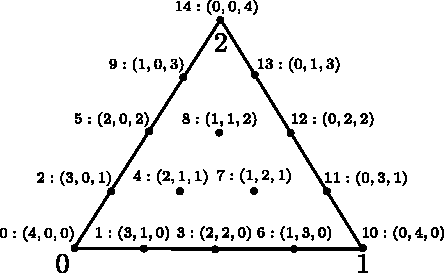
\includegraphics[width=0.5\textwidth]{figures/tridof-4.pdf}
\caption{The interpolation points of $\mathbb T^2_4$ and their
linear indices and multi-indexs. }
\label{fig:interpointk4}
\end{figure}

By this geometric embedding, we can apply operators to the geometric simplex $T$. For example, $\mathcal X_{\mathring{T}}$ denotes the set of interpolation points in the interior of $T$ and $\mathcal X_{\partial T}$ is the set of interpolation points on the boundary of $T$. 


\subsection{Sub-simplexes and sub-simplicial lattices}
Following~\cite{ArnoldFalkWinther2009}, let $\Delta(T)$ denote all the subsimplices of $T$, while $\Delta_{\ell}(T)$ denotes the set of subsimplices of dimension $\ell$ for $\ell=0,\ldots, n$. 
%The cardinality of $\Delta_{\ell}(T)$ is $\displaystyle{n+1\choose \ell+1}$. 
%Elements of $\Delta_0(T) = \{{\bs x}_0, \ldots, {\bs x}_n\}$ are $n+1$ vertices of $T$ and $\Delta_n(T) = \{T\}$. 
The capital letter $F$ is reserved for an $(n-1)$-dimensional face of $T$ and $F_i\in\Delta_{n-1}(T)$ denotes the face opposite to ${\bs x}_i$ for $i=0,1,\ldots, n$.

%It is the combinatory structure of the simplex that plays an important role in the construction. 
For a sub-simplex $f\in \Delta_{\ell}(T)$, following~\cite{Chen;Huang:2022FEMcomplex3D}, we will overload the notation $f$ for both the geometric simplex and the algebraic set of indices. Namely $f = \{f(0), \ldots, f(\ell)\}\subseteq \{0, 1, \ldots, n\}$ and 
$$
f ={\rm Convex}({\bs x}_{f(0)}, \ldots, {\bs x}_{f(\ell)}) \in \Delta_{\ell}(T)
$$
is the $\ell$-dimensional simplex spanned by the vertices ${\bs x}_{f(0)}, \ldots, {\bs x}_{f( \ell)}$.
%There is a one-to-one mapping
%$$
%\Sigma(0 : \ell, 0: n)\to \Delta_{\ell}(T): \sigma \to f_{\sigma}.
%$$
%With a little bit abuse of notation, we also use $f$ for the index $\sigma$. That is for an $f\in \Delta_{\ell}(T)$, we treat $f\in \Sigma(0 : \ell, 0: n)$ so that $
%f=\left[{\bs x}_{f(0)}, \ldots, {\bs x}_{f(\ell)}\right]\in \Delta_{\ell}(T).$
%Then
%$$
%\lambda_{f}^{\alpha_f}: = \lambda_{\sigma}^{\alpha_{\sigma}} = \lambda_{\sigma(0)}^{\alpha_{\sigma(0)}} \ldots \lambda_{\sigma(\ell)}^{\alpha_{\sigma(\ell)}} = \lambda_{f(0)}^{\alpha_{f(0)}} \ldots \lambda_{f(\ell)}^{\alpha_{f(\ell)}},
%$$
%which shows direct relation to $f$ without resort to $\sigma$. When we want to emphasize the dimension of $f$, we write $f^{\ell}$ for an $f\in \Delta_{\ell}(T)$.

If $f \in \Delta_{\ell}(T)$, then $f^{*} \in \Delta_{n- \ell-1}(T)$ denotes the sub-simplex of $T$ opposite to $f$. When treating $f$ as a subset of $\{0, 1, \ldots, n\}$, $f^*\subseteq \{0,1, \ldots, n\}$ so that $f\cup f^* = \{0, 1, \ldots, n\}$, i.e., $f^*$ is the complement of set $f$. Geometrically,
$$
f^* ={\rm Convex}({\bs x}_{f^*(1)}, \ldots, {\bs x}_{f^*(n-\ell)}) \in \Delta_{n- \ell-1}(T)
$$
is the $(n- \ell-1)$-dimensional simplex spanned by vertices not contained in $f$. 


Given a sub-simplex $f\in \Delta_{\ell}(T)$, through the geometric embedding $f \hookrightarrow T$, we define the prolongation/extension operator $E: \mathbb T^{\ell}_k \to \mathbb T^{n}_k$ as follows:
\begin{equation}\label{eq:Ealpha}
E(\alpha)_{f(i)} = \alpha_{i}, i=0,\ldots, \ell, \quad \text{ and } E(\alpha)_j = 0, j\not\in f.
\end{equation}
Take $f = \{ 1, 3, 4\}$ for example,
then the extension $ E(\alpha)= (0, \alpha_{0}, 0, \alpha_{1}, \alpha_{2}, \ldots, 0)$ for 
$\alpha = ( \alpha_{0},\alpha_{1},\alpha_{2})\in \mathbb T^{\ell}_k(f)$. 
With a slight abuse of notation, for a node $\alpha_f\in \mathbb T^{\ell}_k(f)$, we still use the same notation $\alpha_f\in \mathbb T^{n}_k(T)$ to denote such extension. 
The geometric embedding $\bs x_{E(\alpha)}\in f$ which justifies the notation $\mathbb T^{\ell}_k(f)$ and its geometric embedding will be denoted by $\mathcal X_f$, which consists of interpolation points on $f$. $\mathbb T^{\ell}_k(\mathring{f})$ is the set of lattice points whose geometric embedding is in the interior of $f$, i.e., $\mathcal X_{\mathring{f}}$. 


%\subsection{Bubble polynomial}
The Bernstein representation of polynomial of degree $k$ on a simplex $T$ is
$$
\mathbb P_k(T) := \textrm{span} \{ \lambda^{\boldsymbol \alpha} = \lambda_{0}^{\alpha_0}\lambda_{1}^{\alpha_1}\ldots \lambda_{n}^{\alpha_n}, \alpha\in \mathbb T_k^{n}\}.
$$
%In the Bernstein form, for an $f_{\sigma}\in \Delta_{\ell}(T)$, 
%$$
%\mathbb P_k(f_{\sigma}) =\{ \lambda_{\sigma}^{\alpha} = \lambda_{\sigma(0)}^{\alpha_0}\lambda_{\sigma(1)}^{\alpha_1}\ldots \lambda_{\sigma(\ell)}^{\alpha_{\ell}},  \alpha \in \mathbb T_k^{\ell}\}.
%$$
%Through the natural extension defined by the barycentric coordinate, $\mathbb P_k(f_{\sigma})\subseteq \mathbb P_k(T)$. 
The bubble polynomial of $f$ is a polynomial of degree $\ell + 1$:
$$
b_f: = \lambda_{f} = \lambda_{f(0)}\lambda_{f(1)}\ldots \lambda_{f(\ell)}\in \mathbb P_{\ell + 1}(f).
$$

%The following result can be found in~\cite{Chen;Huang:2021Geometric}. For completeness, we include here. 
%\begin{lemma}\label{lm:bf}
%Let $f\in \Delta_{\ell}(T)$ with $\ell \geq 1$. 
%For $e\in \Delta_{m}(T)$ with $m\leq \ell$ and $e\neq f$, then $b_f|_{e} = 0$. And $b_f|_F = 0$ for face $F\in \Delta_{n-1}(T), f\not\subseteq F$. 
%\end{lemma}
%\begin{proof}
%Take any $e\in \Delta_{m}(T)$ with $m\leq \ell$ and $e\neq f$ when $m=\ell$. We claim $f\cap e^* \neq \varnothing$. Assume $f\cap e^* = \varnothing$. Then $\Delta_0(f^*)\cup \Delta_0(e) = \{0,1,\ldots, n\}$ and thus $f\subseteq e$ which contradicts with either $m< \ell$ or $e\neq f$. 
%
%As $f\cap e^* \neq \varnothing$, then $b_f$ contains $\lambda_i$ for some $i\in e^*$ and consequently $b_f|_e = 0$. 
%
%Similarly $f\not\subseteq F$ implies $b_f$ contains $\lambda_i$ for some $i\not\in F$ and consequently $b_f|_F = 0$. 
%\end{proof}
 
\subsection{Triangulation}
Let $\Omega$ be a polyhedral domain in $\mathbb R^n$, $n\geq1$. A geometric
triangulation $\mathcal T_h$ of $\Omega$ is a set of $n$-simplices such that
$$
\cup_{T\in \mathcal T_h} T = \Omega, \quad \mathring T_i \cap \mathring T_j =
\emptyset, \ \forall\ T_i, T_j \in \mathcal T_h, T_i \neq T_j.
$$
The subscript $h$ denotes the diameter of each element and can be understood as a piecewise constant function on $\mathcal T_h$. 
A  triangulation is conforming if the intersection of two simplexes are common lower dimensional sub-simplex. We shall restrict to conforming triangulations in this paper. 

The interpolation points on a conforming triangulation $\mathcal T_h$ is 
\begin{equation}\label{eq:Xunion}
\mathcal X = \bigcup_{T\in \mathcal T_h}\mathcal X_{T}.
\end{equation}
Note that a lot of duplications exist in \eqref{eq:Xunion}. A direct sum of the interpolation set is given by 
\begin{equation}\label{eq:Xsum}
\mathcal X = \Oplus_{\ell = 0}^n \Oplus_{f\in \Delta_{\ell}(\mathcal T_h)} \mathcal X_{\mathring{f}},
\end{equation}
where $\Delta_{\ell}(\mathcal T_h)$ denotes the set of $\ell$-dimensional subsimplices of $\mathcal T_h$.
In implementation, computation of local matrices on each simplex is based on \eqref{eq:Xunion} while to assemble a matrix equation, \eqref{eq:Xsum} should be used. As Lagrange element is globally continuous, the indexing of interpolation points on vertices, edges, faces should be unique and a mapping from the local index to the global index is needed. The index mapping from \eqref{eq:Xunion} to \eqref{eq:Xsum} will be discussed in Section \ref{sec:implementation}. 




\section{Geometric Decompositions of Lagrange Elements}\label{sec:lagrange}
In this section, we present a geometric decomposition for Lagrange finite elements on $n$-dimensional simplices. We introduce the concept of Lagrange interpolation basis functions, where function values at interpolation points serve as degrees of freedom. 

\subsection{Geometric decomposition}
For the polynomial space $\mathbb P_k(T)$ with $k\geq 1$ on an $n$-dimensional simplex $T$, we have the following geometric decomposition of Lagrange element~\cite[(2.6)]{ArnoldFalkWinther2009} and a proof can be found in~\cite{Chen;Huang:2021Geometric}. The integral at a vertex is understood as the function value at that vertex and $\mathbb P_k({\bs x}) = \mathbb R$.

\begin{theorem}[Geometric decomposition of Lagrange element]\label{thm:Lagrangedec}
For the polynomial space $\mathbb P_k(T)$ with $k\geq 1$ on an $n$-dimensional simplex $T$, we have the following decomposition %of shape functions
\begin{align}
\label{eq:Prdec}
\mathbb P_k(T) &= \Oplus_{\ell = 0}^n\Oplus_{f\in \Delta_{\ell}(T)} b_f\mathbb P_{k - (\ell +1)} (f).
\end{align}
The function $u\in \mathbb P_k(T)$ is uniquely determined by DoFs
\begin{equation}\label{eq:dofPr}
\int_f u \, p \dd s, \quad \quad~p\in \mathbb P_{k - (\ell +1)} (f), f\in \Delta_{\ell}(T), \ell = 0,1,\ldots, n.
\end{equation}
\end{theorem}

%A proof of the unisolvence can be found in~\cite{Chen;Huang:2021Geometric}.
%\begin{theorem}\label{th:Lagrange}
%\begin{align}
%\label{eq:Prdec}
%\mathbb P_k(T) &= \Oplus_{\ell = 0}^n\Oplus_{f\in \Delta_{\ell}(T)} b_f\mathbb P_{k - (\ell +1)} (f).
%\end{align}
%The function $u\in \mathbb P_k(T)$ is uniquely determined by DoFs
%\begin{equation}\label{eq:dofPr}
%\int_f u \, p \dd s \quad \forall~p\in \mathbb P_{k - (\ell +1)} (f), f\in \Delta_{\ell}(T), \ell = 0,1,\ldots, n.
%\end{equation}
%\end{theorem}


Introduce the bubble polynomial space of degree $k$ on a sub-simplex $f$ as
$$
\mathbb B_{k}( f) := b_f\mathbb P_{k - (\ell +1)} (f), \quad f\in \Delta_{\ell}(T), 1\leq \ell \leq n.
$$
It is called a bubble space as
$$
\tr^{\grad} u := u|_{\partial f} = 0, \quad u\in \mathbb B_{k}( f).
$$
%The notation $ \mathbb B_{k}( f)$ can be naturally extended to vertices: $\mathbb B_{k}({\bs x}) = \spa \{\lambda_{{\bs x}}\}$. 
Then we can write \eqref{eq:Prdec} as
\begin{equation}\label{eq:Lagdecbubble}
\mathbb P_k(T) = \mathbb P_1(T)\oplus \Oplus_{\ell = 1}^n\Oplus_{f\in \Delta_{\ell}(T)} \mathbb B_{k}( f).
\end{equation}
That is a polynomial of degree $k$ can be decomposed into a linear polynomial plus bubbles on edges, faces, and all sub-simplexes. 

Based on a conforming triangulation $\mathcal T_h$, the $k$-th order Lagrange finite element space $V_k^{\rm L}(\mathcal T_h)$ is defined as 
$$
V_k^{\rm L}(\mathcal T_h) = \{ v\in C(\Omega): v|_{T}\in \mathbb P_k(T),  T\in \mathcal T_h, \text{ and DoFs \eqref{eq:dofPr} are single valued}\},
$$
and will have a geometric decomposition
\begin{equation}\label{eq:VLdec}
V_k^{\rm L}(\mathcal T_h) = V_1^{\rm L}(\mathcal T_h) \,\oplus\, \Oplus_{\ell = 1}^n \Oplus_{f\in \Delta_{\ell}(\mathcal T_h)} \mathbb B_k(f).
\end{equation}
Here we extend the polynomial on $f$ to each element $T$ containing $f$ by the Bernstein form and extension of multi-index; see $E(\alpha)$ defined in \eqref{eq:Ealpha}. Consequently the dimension of $V_k^{\rm L}$ is
$$
V_k^{\rm L}(\mathcal T_h) = \sum_{\ell = 0}^n |\Delta_{\ell}(\mathcal T_h)| { k - 1 \choose \ell},
$$
where $|\Delta_{\ell}(\mathcal T_h)|$ is the cardinality of  number of $\Delta_{\ell}(\mathcal T_h)$, i.e., the number of $\ell$-dimensional simplices in $\mathcal T_h$. We understand ${ k - 1 \choose \ell} = 0$ if $\ell > k-1$. That is the degree of the polynomial dictates the dimension of the sub-simplex in the geometric decompositions \eqref{eq:Prdec} and \eqref{eq:VLdec}. 
%For example, with $k=2$, the summation includes only edge bubbles and excludes face bubbles and higher dimensions. Despite this, the full summation notation $\Oplus_{\ell=0}^n$ is retained for simplicity, with the implicit understanding that the range of non-zero sub-spaces will automatically truncate the limits.

%\begin{remark} 
%For spaces associated to vertices, it can be changed to
%$$
%\spa \{\lambda_{i}^{r}, i=0, 1,\ldots, n\},
%$$
%which is consistent with the Bernstein representation $\lambda^{\alpha}$. 
%\end{remark}

The geometric decomposition \eqref{eq:Prdec} can be naturally extended to vector Lagrange
elements. For $k\geq 1$, define 
\begin{equation*}
\mathbb B_{k}^n(f) := b_f\mathbb P_{k - (\ell +1)} (f)\otimes \mathbb R^n.
\end{equation*}
%
Clearly we have
\begin{align}\label{eq:Pkvecdec}
\mathbb P_k^n(T)&= \mathbb P_1^n(T)\oplus \Oplus_{\ell = 1}^n\Oplus_{f\in \Delta_{\ell}(T)} \mathbb B_{k}^n(f).
\end{align}
For an $f\in \Delta_{\ell} (T)$, we choose a $t-n$ coordinate 
$\{\bs t_i^f, \bs n_j^f, i=1, \dots, \ell, j = 1, \dots, n-\ell\}$ so that
\begin{itemize}
\item $\mathscr T^f := \textrm{span}\{ \bs t_1^f, \ldots, \bs t_{\ell}^f \}, $ is the tangential plane of $f$;

\item $\mathscr{N}^f :=  \textrm{span}\{ \bs n_1^f, \ldots, \bs n_{n - \ell}^f \} $ is the normal plane of $f$. 
\end{itemize}
%Thus $\mathscr T^f$ is the tangent plane of $f$ and $\mathscr{N}^f$ is the normal plane. 
%For $r\geq 1$, define
%\begin{equation*}%\label{eq:fbubble}
%\mathbb B_k(f) \mathscr T^f_k( T) := \left \{\sum_{i=1}^{\ell} u_i^f \bs t_i^f: u_i^f \in \mathbb B_k(f) \right \},
%\end{equation*}
%\begin{equation*}
%\mathscr{N}^f_k( T) := \left \{\sum_{i=1}^{n-\ell} u_i^f \bs n_i^f:  u_i^f \in \mathbb B_k(f) \right \}.
%\end{equation*}
%We can also write 
%$$
%\mathscr T^f_k(T) = b_f\mathbb P_{k - (\ell +1)} (f)\otimes \mathscr T_0^f, \quad \mathscr{N}^f_k( T) = b_f\mathbb P_{k - (\ell +1)} (f)\otimes \mathscr{N}_0^f.
%$$
%Note that $\mathscr T^f_k( T), \mathscr{N}^f_k( T)\subseteq \mathbb P_k^n(T)$ for $r\geq 1$, while for $r=0$, $\mathscr T_0^f$ and $\mathscr{N}_0^f$ are independent of $T$. 
%
When $\ell = 0$, i.e., for vertices, no tangential component, and for $\ell = n$, no normal component. 
We abbreviate $\bs n_1^F$ as $\bs n_F$ for $F\in\Delta_{n-1}(T)$, and $\bs t_1^e$ as $\bs t_e$ for $e\in\Delta_{1}(T)$.
We have the trivial decompositions
\begin{equation}\label{eq:tndec}
\mathbb R^n = \mathscr T^{f}\oplus \mathscr N^f, \quad \mathbb B_{k}^n(f) = \left [\mathbb B_{k}(f)\otimes \mathscr T^{f}\right ]\Oplus \left [\mathbb B_{k}(f)\otimes\mathscr N^f \right ].
\end{equation}
%
Restricted to an $\ell$-dimensional sub-simplex $f\in \Delta_{\ell}(T)$,  define
$$ 
\mathbb B_{k}^{\ell}(f) := \mathbb B_k(f) \otimes \mathscr{T}^f,
$$ 
which is a space of $\ell$-dimensional vectors on the tangential space $\mathscr{T}^f$ with vanishing trace $\tr^{\grad}$ on $\partial f$. 
%As a corollary of Theorem \ref{thm:Lagrangedec} and $t-n$ decomposition \eqref{eq:tndec}, we have the following decomposition of the vector Lagrange elements. 
%We then rewrite the decomposition \eqref{eq:Pkvecdec} as
%\begin{align}\label{eq:Prvecdec2}
%\mathbb P_k^n(T)=\mathbb P_1^n(T) \,\oplus \Oplus_{\ell = 1}^{n}\Oplus_{f\in
%\Delta_{\ell}(T)} \left [ \mathbb B_k^{\ell}(f) \oplus (\mathbb B_k(f) \otimes \mathscr{N}^f) \right ].
%\end{align}

%\begin{corollary} \label{lm:vecLdec}
%Let $k\geq 1$ be an integer. For each $f\in \Delta_{\ell} (T)$, we choose a $t-n$ basis $\{\bs t_i^f, \bs n_j^f, i=1, \dots, \ell, j = 1, \dots, n-\ell\}$.
%Then a function $\bs u \in \mathbb P_k(T; \mathbb R^n)$ is uniquely determined by the DoFs
%\begin{subequations}\label{eq:dofvec}
%\begin{align}
%\label{eq:dofvectort}
%\int_f (\bs u\cdot \bs t_i^f)\ p \dd s,& \, i=1,\ldots, \ell, p\in \mathbb P_{k - (\ell +1)} (f), f\in \Delta_{\ell}(T), \ell = 1,\ldots, n,\\
%\label{eq:dofvectorn}
%\int_f (\bs u\cdot \bs n_j^f)\ p \dd s, & \, j=1,\ldots, n - \ell, p\in \mathbb P_{k - (\ell +1)} (f), f\in \Delta_{\ell}(T), \ell = 0,\ldots, n-1.
%\end{align}
%\end{subequations}
%%for all $p\in \mathbb P_{k - (\ell +1)} (f), f\in \Delta_{\ell}(T), \ell = 0,1,\ldots, n$.
%\end{corollary}

When move to a triangulation $\mathcal T_h$, we shall call a basis of $\mathscr T^f$ or $\mathscr N^f$ is global if it depends only on $f$ not the element $T$ containing $f$. Otherwise it is called local and may vary in different elements. 


%We prove it is indeed surjective. 
%\begin{lemma}\label{lem:trdivonto}
%For integer $r\geq 1$, the mapping ${\rm tr}^{\div}: \mathbb P_k^n(T) \to \mathbb P_{k}(\partial T)$ is onto. 
%\end{lemma}

% Indeed we can give a geometric decomposition of $\mathbb B_k(\div, T)$. In the sequel, $\mathbb R^{\ell}(f)$ denotes the tangent plane of $F$ which can be naturally embedded into $\mathbb R^n$ through $F$. The vector function
%$$
%b_f\mathbb P_{k - (\ell +1)} (f)\otimes \mathbb R^{\ell}(f)
%$$
%can be identified with a differential form in $\mathbb P_k\Lambda^{n-1}$ through
%$$
%\prox^{-1} ({\rm Ext}(b_f\mathbb P_{k - (\ell +1)} (f)) \otimes {\rm Ext}(\mathbb R^{\ell}(f))).
%$$
%We will stick to the simpler vector function notation. 

\subsection{Lagrange interpolation basis functions}\label{sec:lagrangebasis}
Previously DoFs \eqref{eq:dofPr} are given by moments on sub-simplexes. Now we present a set of DoFs as function values on the interpolation points and give its dual basis for the $k$-th order Lagrange element on an $n$-simplex.

\begin{lemma}[Lagrange interpolation basis functions~\cite{nicolaides1972class}]\label{le:li}
A basis function of the $k$-th order Lagrange finite element space on $T$ is:
$$
\phi_{\boldsymbol \alpha}(\boldsymbol x) = 
\frac{1}{\boldsymbol \alpha!} 
\prod_{i=0}^{n}\prod_{j =0}^{\alpha_i - 1} (k\lambda_i(\boldsymbol x) - j), \quad 
\boldsymbol \alpha \in \mathbb T^n_k,
$$
with the DoFs defined as the function value at the interpolation points:
$$
N_{\bs \alpha} (u) = u(\boldsymbol x_{\alpha}), \quad \boldsymbol x_{\alpha} \in \mathcal X_{T}.
$$
\end{lemma}
\begin{proof}
It is straightforward to verify the duality of the basis and DoFs 
$$
N_{\bs \beta}(\phi_{\bs \alpha}) = \phi_{\bs \alpha}(\bs x_{\beta}) = \delta_{\bs \alpha,\bs \beta} = 
\begin{cases}
1& \text{ if } \bs \alpha = \bs \beta\\
0 & \text{ otherwise }
\end{cases}.
$$
As $$| \mathbb T^{n}_k | = {n + k \choose k} = \dim \mathbb P_k(T),$$ $\{\phi_{\boldsymbol \alpha}, \bs \alpha\in  \mathbb T^{n}_k\}$ is a basis of $\mathbb P_k(T)$ and $\{N_{\boldsymbol \alpha}, \bs \alpha\in  \mathbb T^{n}_k\}$ is a basis of the dual space $\mathbb P_k^*(T)$.
\end{proof}
%Note that the basis functions can be also indexed by $R_n(\boldsymbol \alpha)$.  

Given a triangulation $\mathcal T_h$ and
degree $k$, recall that
$$
\mathcal X_{\mathcal T_h} = \bigcup_{T\in\mathcal T_h} \mathcal X_T = \Oplus_{\ell = 0}^n \Oplus_{f\in \Delta_{\ell}(\mathcal T_h)} \mathcal X_{\mathring{f}}.
$$
Denote by
$$
\mathbb T_k^n(\mathcal T_h) := \Oplus_{\bs x_i\in \Delta_0(\mathcal T_h)}\mathbb T_k^{0}(\bs x_i) \oplus \Oplus_{\ell = 1}^n \Oplus_{f\in \Delta_{\ell}(\mathcal T_h)} \mathbb T_k^{\ell}(\mathring{f}).
$$
For a lattice $\alpha \in \mathbb T_k^{\ell}(\mathring{f})$, we use extension operator $E$ defined in \eqref{eq:Ealpha} to extend $\alpha$ to each simplex $T$ containing $f$. We also extend the polynomial on $f$ to $T$ by the Bernstein form.

\begin{theorem}[DoFs of Lagrange finite element on $\mathcal T_h$]
A basis for the $k$-th Lagrange finite element space $V_k^{\rm L}(\mathcal T_h)$ 
is 
$$\{\phi_{\boldsymbol \alpha}, \bs \alpha\in  \mathbb T^{n}_k(\mathcal T_h)\}$$ with DoFs
$$
N_{\bs \alpha} (u) = u(\boldsymbol x_{\alpha}), \quad \boldsymbol x_{\alpha} \in \mathcal X_{\mathcal T_h}.
$$
\end{theorem}
\begin{proof}
For $F\in \Delta_{n-1}(\mathcal T_h)$, thanks to Lemma~\ref{le:li}, $\phi_{\boldsymbol \alpha}|_F$ is uniquely determined by DoFs $\{u(\boldsymbol x_{\alpha}), \boldsymbol x_{\alpha} \in \mathcal X_{F}\}$ on face $F$, hence $\phi_{\boldsymbol \alpha}\in V_k^{\rm L}(\mathcal T_h)$. Clearly the cardinality of $\{\phi_{\boldsymbol \alpha}, \bs \alpha\in  \mathbb T^{n}_k(\mathcal T_h)\}$ is same as the dimension of space $V_k^{\rm L}(\mathcal T_h)$. Then we only need to show these functions are linearly independent,  which follows from the fact $N_{\bs \beta}(\phi_{\bs \alpha}) = \phi_{\bs \alpha}(\bs x_{\beta}) = \delta_{\bs \alpha,\bs \beta}$ for $\bs \alpha, \bs \beta\in\mathbb T^{n}_k(\mathcal T_h)$.
\end{proof}

We now generalize the basis for a scalar Lagrange element to a vector Lagrange element.
For an interpolation point $\bs x\in \mathcal X_{T}$, let $\{\bs e_i^{\bs x}, i=0,\ldots, n-1\}$ be a basis of $\mathbb R^n$, and its dual basis is denoted by $\{\hat{\bs e}_i^{\bs x}, i=0,\ldots, n-1\}$, i.e.,
$$
(\hat{\bs e}_i^{\bs x}, \bs e_j^{\bs x}) = \delta_{i,j}.
$$
When $\{\bs e_i^{\bs x}, i=0,\ldots, n-1\}$ is orthonormal, its dual basis is itself. 
% In general, we can always choose an orthonormal basis for the tangential plane $\mathscr T^f$ but for the normal plane $\mathscr N^f$, we can use Lemma \ref{lm:dualnormal} to find the dual basis. 

\begin{corollary}\label{cor:basisfunctions}
    A polynomial function $\bs u \in \mathbb P_k^n(T)$ can be uniquely determined by the DoFs:
  $$
N^i_{\bs \alpha }(\bs u):=  \bs u(\bs x_{\bs \alpha})\cdot \bs e^{\bs x_{\bs \alpha}}_i, \quad \bs x_{\bs \alpha} \in \mathcal X_{T}, i = 0,\ldots, n-1.
  $$
  The basis function on $T$ dual to this set of DoFs can be 
  explicitly written as:
  $$
  \bs{\phi}_{\bs \alpha}^i(\bs x) = 
  \phi_{\bs\alpha}(\bs x) \hat{\bs e}^{\bs x_{\bs \alpha}}_i, \quad 
  \boldsymbol \alpha \in \mathbb T^n_k, i = 0, \ldots, n-1.
  $$
\end{corollary}
 \begin{proof}
It is straightforward to verify the duality
$$
N^j_{\bs \beta }(\bs{\phi}_{\bs \alpha}^i) =   \bs{\phi}_{\bs \alpha}^i(\bs x_{\beta}) \cdot \bs e^{\bs x_{\beta}}_j  =   \phi_{\bs \alpha}(\bs x_{\beta}) \hat{\bs e}^{\bs x_{\bs \alpha}}_i \cdot \bs e^{\bs x_{\beta}}_j  = \delta_{i,j} \delta_{\bs \alpha,\bs \beta},
$$ 
for $\bs \alpha, \bs \beta\in  \mathbb T^n_k, i,j = 0,\ldots, n-1.$
\end{proof}
If the basis $\{\bs e_i^{f}, i=0,\ldots, n-1\}$ is global in the sense that it is independent of element $T$ containing $\bs x$, we get the continuous vector Lagrange elements. Choose different basis will give different continuity.

\section{Geometric Decompositions of Face Elements}\label{sec:facefem}
Define $H(\div, \Omega):=\{\bs v\in L^2(\Omega;\mathbb R^n): \div \bs v\in L^2(\Omega)\}.$ For a subdomain $K\subseteq \Omega$, the trace operator for the div operator is
$$
{\rm tr}_K^{\div} \boldsymbol v = \boldsymbol n\cdot \boldsymbol v|_{\partial K} \quad \textrm{ for }\;\;\boldsymbol{v}\in H(\div, \Omega),
$$
where $\bs n$ denotes the outwards unit normal vector of $\partial K$. 
Given a triangulation $\mathcal T_h$ and a piecewise smooth function $\bs u$, it is well known that $\bs u\in H(\div, \Omega)$ if and only if $\bs n_F \cdot \bs u$ is continuous across all faces $F\in \Delta_{n-1}(\mathcal T_h)$, which can be ensured by having DoFs on faces. %where $\bs n_F$ is a global normal vector of $F$. 
An $H(\div)$-conforming finite element is thus also called a face element.

%We shall consider Brezzi-Douglas-Marini (BDM) element~\cite{BrezziDouglasMarini1985} or second family of N\'ed\'elec face element~\cite{Nedelec1986,BrezziDouglasDuranFortin1987,ArnoldFalkWinther2006} whose shape function space is full polynomial space $\mathbb P_k^n$. 

\subsection{Geometric decomposition}
Define the polynomial $\div$ bubble space
$$
\mathbb B_k(\div, T) = \ker(\tr_T^{\div})\cap \mathbb P_k^n(T).
$$
Recall that $\mathbb B_{k}^{\ell}(f) = \mathbb B_k(f) \otimes \mathscr{T}^f$ consists of bubble polynomials on the tangential plane of $f$. For $\bs u\in \mathbb B_{k}^{\ell}(f)$, as $\bs u$ is on the tangent plane, $\bs u\cdot \bs n_F = 0$ for $f\subseteq F$. When $f\not\subseteq F$, $b_f|_F =0$. So $\mathbb B_{k}^{\ell}(f)\subseteq \mathbb B_k(\div, T)$
for $k\geq 2$ and $\dim f \geq 1$. In~\cite{Chen;Huang:2021Geometric}, 
we have proved that the $\div$-bubble polynomial space has the following decomposition.
\begin{lemma}\label{lem:divbubble}
For $k\geq 2$,
$$
\mathbb B_k(\div, T) = \Oplus_{\ell=1}^n\Oplus_{f\in\Delta_{\ell}(T)}\mathbb B_{k}^{\ell}(f).
$$
\end{lemma}
Notice that as no tangential plane on vertices, there is no $\div$-bubble associated to vertices and consequently the degree of a $\div$-bubble polynomial is greater than or equal to $2$. 
%
%The volume Lagrange bubble $\mathbb B_k^n(T)$ has no contribution to the trace. 
Next we present two geometric decompositions of a $\div$-element. 

%This implies $\bs u({\bs x})=\bs0$ for ${\bs x}\in\Delta_0(T)$ and $\bs u\in\mathbb B_k(\div, T)$. And we have (cf. Lemma~3.6 in~\cite{ChenHuang2021})
%\begin{equation}\label{eq:divbubbleonto}
%\div \mathbb B_k(\div, T)=\mathbb P_{k-1}(T)/\mathbb R.
%\end{equation}

%For $F\in\Delta_{n-1}(T)$, \Oplus_{F\in\Delta_{n-1}(T)}
%$$
%\mathbb B_k(\div; F) = \mathbb P_1(F)\bs n_F\oplus \Oplus_{\ell=1}^{n-1}\Oplus_{f\in\Delta_{\ell}(T), f\subseteq F}\mathbb B_{k}( f)\bs n_F.
%$$
\begin{theorem}\label{thm:BDMgeodecomp}
For $k\geq 1$, we have
\begin{align}
\label{eq:divpolynomialdecomp}
\mathbb P_k^n(T) &= \mathbb P_1^n(T) \oplus \big(\Oplus_{\ell=1}^{n-1}\Oplus_{f\in\Delta_{\ell}(T)}(\mathbb B_{k}( f) \otimes \mathscr{N}^f)\big)\oplus \mathbb B_k(\div, T),\\
\label{eq:divpolynomialdecomp2}
\mathbb P_k^n(T) &= \big(\Oplus_{F\in\Delta_{n-1}(T)} \left ( \mathbb P_k(F)\bs n_F \right )\big)\oplus \mathbb B_k(\div, T).
\end{align}
\end{theorem}
\begin{proof}
The first decomposition \eqref{eq:divpolynomialdecomp} is a rearrangement of \eqref{eq:Pkvecdec} by merging the tangential component $\mathbb B_{k}^{\ell}( f) $ into the bubble space $\mathbb B_k(\div, T)$. 

Next we prove the decomposition \eqref{eq:divpolynomialdecomp2}.
%
For an $\ell$-dimensional, $0\leq \ell\leq n-1$, sub-simplex $f\in\Delta_{\ell}(T)$, we choose the $n-\ell$ face normal vectors $\{\bs n_{F}: F\in \Delta_{n-1}(T), f\subseteq F\}$ as the basis of $\mathscr{N}^f$. Therefore  we have
$$
\mathbb B_{k}( f) \otimes \mathscr{N}^f =\Oplus_{F\in \Delta_{n-1}(T), f\subseteq F}\mathbb B_{k}( f)\bs n_F.
$$
Then \eqref{eq:divpolynomialdecomp} becomes
\begin{equation*}%\label{eq:divpolynomialdecomp1}
\mathbb P_k^n(T) = \mathbb P_1^n(T) \oplus \big(\Oplus_{\ell=1}^{n-1}\Oplus_{f\in\Delta_{\ell}(T)}\Oplus_{F\in \Delta_{n-1}(T), f\subseteq F}\mathbb B_{k}( f)\bs n_F\big)\oplus \mathbb B_k(\div, T).
\end{equation*}
At a vertex $\texttt{v}$, we choose $\{\bs n_{F}: F\in \Delta_{n-1}(T), \texttt{v}\subseteq F\}$ as the basis of $\mathbb R^n$ and write 
\begin{align*}  
\mathbb P_1^n(T) 
%&= \Oplus_{{\bs x}\in \Delta_{0}(T)} {\rm span}\{\lambda_{{\bs x}}\}\otimes \mathscr{N}^{{\bs x}}\\
&= \Oplus_{{\bs x}\in \Delta_{0}(T)}\Oplus_{F\in\Delta_{n-1}(T), {\bs x}\in\Delta_0(F)}{\rm span}\{ \lambda_{{\bs x}}\bs n_F\} \\
&= \Oplus_{F\in\Delta_{n-1}(T)}\Oplus_{{\bs x}\in \Delta_{0}(F)}{\rm span}\{ \lambda_{{\bs x}}\bs n_F\}\\
&= \Oplus_{F\in\Delta_{n-1}(T)} \mathbb P_1(F)\bs n_F.
\end{align*}
Then by swapping the ordering of $f$ and $F$ in the direct sum, i.e.,
$$
\Oplus_{\ell=1}^{n-1}\Oplus_{f\in\Delta_{\ell}(T)}\Oplus_{F\in \Delta_{n-1}(T), f\subseteq F} \to \Oplus_{F\in \Delta_{n-1}(T)}\Oplus_{\ell=1}^{n-1}\Oplus_{f\in\Delta_{\ell}(F)},
$$
and using the decomposition \eqref{eq:Prdec} of Lagrange element, we obtain the decomposition \eqref{eq:divpolynomialdecomp2}.
%
%For edge elements, we distribute $n$-components of a vector at a vertex to $n$ edges co\mc{NN}ected this vertex. 
%Thus decomposition \eqref{eq:divpolynomialdecomp2} follows.
% a vector $\bs u({\bs x}) \in \mathbb R^n$ and can expand in the basis $\{\bs n_{F}: F\in \Delta_{n-1}(T), {\bs x}\subseteq F\}$, i.e.
% $$
% \bs u({\bs x}) = \sum_{F_i\in \Delta_{n-1}(T), {\bs x}\subseteq F_i} (\bs u({\bs x}), \bs l_i)\, \bs n_{F_i},
% $$
% where $\{\bs l_i\}$ is the dual vector of $\{\bs n_{F_i}\}$. Now look at one face $F$, we then have $n$ values at $n$ vertices of $F$, $\{(\bs u({\bs x}), \bs l_F)\, \bs n_{F}, {\bs x}\in F \}$ which will define a function in $\mathbb P_1(F)\bs n_F$. 
% For $i=0,\ldots, n$ and $F\in\Delta_{n-1}(T)$, apparently $\lambda_i\bs n_F\in \mathbb P_1(F)\bs n_F$ if $i\in F$ and  $\lambda_i\bs n_F\in \sum_{f\in\Delta_{n-1}(T), f\neq F}\mathbb P_1(f)\bs n_f^k$ if $i\not\in F$. Hence $\mathbb P_1^n(T)=\sum_{F\in\Delta_{n-1}(T)}\mathbb P_1(F)\bs n_F$, which together with the matching dimensions yields $\mathbb P_1^n(T)=\Oplus_{F\in\Delta_{n-1}(T)}\mathbb P_1(F)\bs n_F$.
\end{proof}

In decomposition \eqref{eq:divpolynomialdecomp}, we single out $\mathbb P_1^n(T)$ to emphasize an $H(\div)$-conforming element can be obtained by adding $\div$-bubble and normal component on sub-simplexes starting from edges. In~\eqref{eq:divpolynomialdecomp2}, we group all normal components facewisely which leads to the classical BDM element.

As $H(\div,\Omega)$-conforming elements require the normal continuity across each $F$, the normal vector $\bs n_F$ is chosen globally. Namely $\bs n_F$ depends on $F$ only. It may coincide with the outwards or inwards normal vector for an element $T$ containing $F$. On the contrary, all tangential basis for $\mathscr T^f$ are local and thus the tangential component are multi-valued and merged to the element-wise div bubble function $\mathbb B_k(\div, T)$. 


%\begin{lemma}[BDM element]\label{lm:bdm}
%The following {\rm DoFs}
%\begin{align}
%%\label{eq:divbdDoF0}
%%(\bs v\cdot \bs n_F)({\bs x}), &\quad  {\bs x}\in \Delta_{0}(\mathcal T_h), F\in \Delta_{n-1}(T),\\
%\label{eq:divbdDoF}
%\int_f (\bs v\cdot \bs n_F)\ p \dd s, &\quad  f\in \Delta_{\ell}(T), F\in \Delta_{n-1}(T), f\subseteq F, \\
%& \quad p\in \mathbb P_{k - (\ell +1)} (f), \ell = 0,\ldots, n-1, \notag\\
%\label{eq:divbubbleDoF}
%\int_f (\bs v\cdot \bs t^f_i)\ p \dd s, &\quad  f\in \Delta_{\ell}(T), i=1,\ldots, \ell , \\
%& \quad p\in \mathbb P_{k - (\ell +1)} (f), \ell = 1,\ldots, n, \notag
%\end{align}
%define a $H(\div)$-conforming space $V_h=\{\bs v_h\in H(\div; \Omega): \bs v_h|_T\in\mathbb P_k^n(T) \;\; \forall~T\in\mathcal T_h\}$.
%\end{lemma}
%
%For BDM element, by the decomposition of Lagrange element, the face DoFs for the trace $\bs v\cdot \bs n_F$ can be merged into 
%\begin{equation}
%\int_F (\bs v\cdot \bs n_F)\ p \dd s, \quad p\in \mathbb P_{k} (F),
%\end{equation}
%and the $\div$ bubble DoFs can be merged into one
%$$
%\int_T \bs v \cdot \bs p \dx \quad \bs p\in \mathbb B_k(\div, T). 
%$$
%But DoF \eqref{eq:divbdDoF}-\eqref{eq:divbubbleDoF} is more friendly for the implementation. One can start from the vector Lagrange element and split into tangential and normal components.   
%%which can be further split into 
%%\begin{align}
%%\label{eq:RT0DoF}
%%\int_F \bs v\cdot \bs n_F \dd s, &\\
%%\label{eq:PrBDMDoF}
%%\int_F \bs v\cdot \bs n_F\, p \dd s &\quad p\in \mathbb P_{k} (F)/\mathbb R.
%%\end{align}
%%Then we have the decomposition
%%\begin{equation}\label{eq:curlpolynomialdecomp3}
%%\mathbb P_k^n(T) = {\rm RT}_0 \oplus \Oplus_{F\in \Delta_{n-1}(T)}((\mathbb P_{k} (F)/\mathbb R) \bs n_F)^* \oplus \mathbb B_k(\div, T).
%%\end{equation}
%
%Based on the decomposition \eqref{eq:divpolynomialdecomp}, we may impose the continuity at vertex to determine $\mathbb P_1^n(T)$ which is known as Sternberg's element~\cite{Stenberg2010}. 
%\begin{lemma}[Stenberg element]
%The following DoFs
%\begin{align*}
%\bs v({\bs x}), &\quad  {\bs x}\in \Delta_{0}(\mathcal T_h),\\
%\int_f (\bs v\cdot \bs n_F)\ p \dd s, &\quad  f\in \Delta_{\ell}(T), F\in \Delta_{n-1}(T), f\subseteq F, \\
%\int_f (\bs v\cdot \bs t^f_i)\ p \dd s, &\quad  f\in \Delta_{\ell}(T), i=1,\ldots, \ell , \\
%& \quad p\in \mathbb P_{k - (\ell +1)} (f), \ell = 1,\ldots, n, \notag
%\end{align*}
%define a $H(\div)$-conforming finite element space being continuous at vertex in $\Delta_{0}(\mathcal T_h)$.
%\end{lemma}
%In general, for each sub-simplex, we can choose either a local or global normal basis and obtain variants of Sternberg element. For each $f\in \Delta_{\ell}(\mathcal T_h)$, we choose a $t-n$ coordinate $\{\bs t_1^f, \ldots, \bs t_{\ell}^f, \bs n_1^f, \ldots, \bs n_{n-\ell}^f \}$. If a basis vector $\bs t_i^f$ or $\bs n_i^f$ depends only on $f$ not on element $T$ containing $f$, we call it {\it global} and otherwise {\em local}. For local $t-n$ basis, the corresponding DoFs are different for different $T$ containing $f$. For a global normal basis, the corresponding DoFs depends only on $f$ and thus the vector is continuous on the normal plane of $f$. 
%\begin{lemma}\label{lm:CHH}
%Let $-1\leq k\leq n-1$. For each $f\in \Delta_{\ell}(\mathcal T_h)$ with $\ell \leq k$, we choose $n-\ell$ normal vectors $\{\bs n^f_{1}, \ldots, \bs n^f_{n-\ell}\}$ depending only on $f$. Then the {\rm DoFs}
%\begin{align*}%\label{eq:vertexDoFTh}
%%\bs v({\bs x}) &\quad  {\bs x}\in \Delta_0(\mathcal T_h),\\
%%\label{eq:faceFDoFTh} 
%\int_f \bs v\cdot \bs n^f_i\, p \dd s, &\quad  p\in \mathbb P_{k-(\ell +1)}(f), f\in \Delta_{\ell}(\mathcal T_h),\\
%&\quad i=1,\ldots, n-\ell, \; \ell = 0,\ldots, k,\\
%%\label{eq:BDMDoFTh} 
%\int_f (\bs v\cdot \bs n_F)\ p \dd s, &\quad  p\in \mathbb P_{k-(\ell +1)}(f),  f\in \Delta_{\ell}(T), \\
%&\quad F\in \Delta_{n-1}(T), f\subseteq F, \; \ell = k+1,\ldots, n-1,\\
%\int_T \bs v\cdot \bs p \dx, &\quad   \bs p\in \mathbb B_k(\div, T),T\in \mathcal T_h,
%\end{align*}
%will determine a space $V^k\subset H(\div,\Omega)$ which is continuous on the normal plane of $f$ for all $f\in \Delta_{\ell}(\mathcal T_h)$ with $\ell \leq k$.
%\end{lemma}
%When $k=0$, it is the original Stenberg element~~\cite{Stenberg2010}, i.e., only
%continuous at vertices. When $k = n-2$, it is the generalization of
%Christiansen-Hu-Hu element~\cite{Christiansen;Hu;Hu:2018finite}. We allow $k=-1$
%to include the BDM element. We refer to~\cite{Chen;Huang:2021Geometric} for the
%proof on the unisolvence.
%Another variant is: for $f\in \Delta_{\ell}(\mathcal T_h), \ell =0,\ldots, n-1$, choose a fixed normal basis. Then the obtained element is normal continuous. 

%\begin{figure}[htbp]
%\begin{center}
%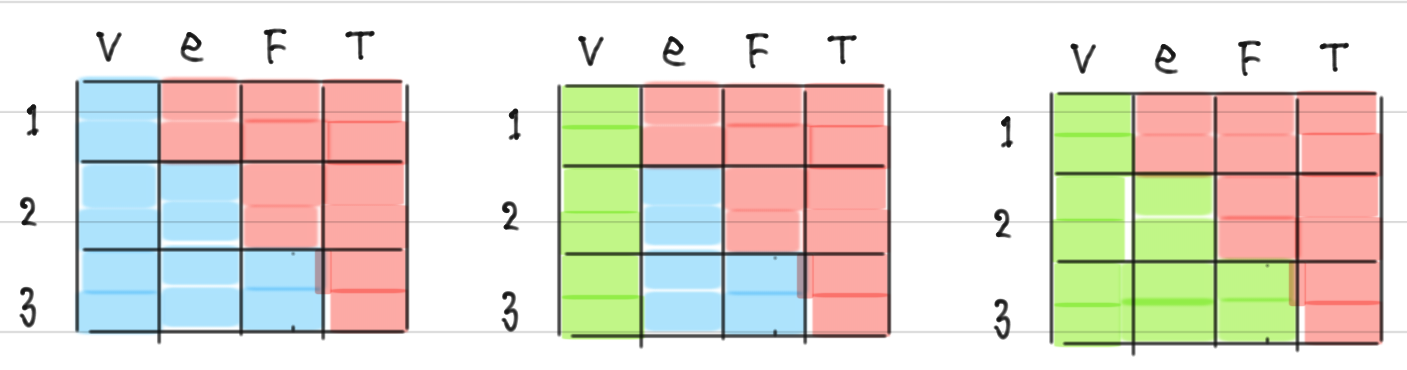
\includegraphics[width=4in]{figures/facegeodec.png}
%\caption{Different continuity of face elements. Left: BDM; Middle: Stenberg; Right: CHH.}
%\label{default}
%\end{center}
%\end{figure}

%\subsection{Tangential-normal decomposition of face elements}
%Given a triangulation $\mathcal T_h$, for each $F\in \Delta_{n-1}(\mathcal T_h)$, we choose a global normal vector $\bs n_F$, i.e., it depends on $F$ only not the element $T$ containing $F$. Given an $f\in \Delta_{\ell}(T)$, we choose $\{\bs n_F, f\subseteq F\in \partial T\}$ as the basis for its normal plane and an arbitrary basis for the tangential plane. We claim the resulting element is the BDM element. 
%
%\begin{theorem}\label{div:equivalentdofs}
%Take $\mathbb P_k^n(T)$ as the shape function space.
%Given an $f\in \Delta_{\ell}(T)$, we choose $\{\bs n_F, f\subseteq F\in \partial T\}$ as the basis for its normal plane and an arbitrary basis $\{\bs t_i^f\}$ for the tangent plane. Then the DoFs 
%\begin{subequations}\label{eq:dofvecdiv}
%\begin{align}
%\label{eq:dofvectorndiv}
%\int_f (\bs u\cdot \bs n_F)\ p \dd s, &\quad  p\in \mathbb P_{k - (\ell +1)} (f), F\in \Delta_{n-1}(T), f\subseteq F, \\
%\label{eq:dofvectortdiv}
%\int_f (\bs u\cdot \bs t_i^f)\ p \dd s,& \quad p\in \mathbb P_{k - (\ell +1)} (f),  i=1,\ldots, \ell, 
%\end{align}
%\end{subequations}
%for all $f\in \Delta_{\ell}(T), \ell = 0,1,\ldots, n$ are equivalent to the BDM element
%\begin{subequations}\label{eq:dofBDM}
%\begin{align}
%\label{eq:vecbdDoF}
%\int_F \bs v\cdot \bs n_F p \dd S, &\quad p\in \mathbb P_k(F), F\in \Delta_{n-1}(T), \\
%%& \quad p\in \mathbb P_{r - (\ell +1)} (f), \ell = 0,1,\ldots, n-1, \notag\\
%\int_T \bs v \cdot \bs p \dx, &\quad \bs p\in \mathbb B_k(\div, T). \label{eq:bubbleDoF}
%\end{align}
%\end{subequations}
%\end{theorem}
%\begin{proof}
%The unisolvence of DoFs \eqref{eq:dofvecdiv} for $\mathbb P_k^n(T)$ follows from Corollary~\ref{lm:vecLdec} and switching the normal basis $\{\bs n_1^f, \ldots, \bs n_{n-\ell}^f\}$ to $\{\bs n_{F}: F\in \Delta_{n-1}(T), f\subseteq F\}$.
%
%By the geometric decomposition \eqref{eq:Prdec} of Lagrange element, we can merge DoFs in \eqref{eq:dofvectorndiv} into DoF \eqref{eq:vecbdDoF}.
%By Lemma~\ref{lem:divbubble}, we can merge DoFs in \eqref{eq:dofvectortdiv} into DoF \eqref{eq:bubbleDoF}.
%\end{proof}

\subsection{A nodal basis for the BDM element}
For the efficient implementation, we employ the DoFs of the function values at interpolation nodes and combine with $t-n$ decompositions to present a nodal basis for the BDM element.  
 
Given an $f\in \Delta_{\ell}(T)$, we choose $\{\bs n_F, F\in \Delta_{n-1}( T), f\subseteq F\}$ as the basis for its normal plane $\mathcal N^f$ and an arbitrary basis $\{ \bs t_i^f, i=1,\ldots, \ell \}$ for the tangential plane. We shall choose  $\{\hat{\bs n}_{F_i}\in \mathcal N^f, i\in f^*\}$ a basis of $\mathcal N^f$  dual to $\{\bs n_{F_i}\in \mathcal N^f, i\in f^*\}$, i.e.,
$$
(\bs n_F, \hat{\bs n}_{F'}) = \delta_{F, F'}, \quad F, F'\in \Delta_{n-1}(T), f\in F\cap F'.
$$
Similarly  choose a basis $\{\hat{\bs t}_i^f\}$ dual to $\{\bs t_j^f\}$.  

We can always choose an orthonormal basis for the tangential plane $\mathscr T^f$ but for the normal plane $\mathscr N^f$ with basis $\{\bs n_{F_i}\in \mathcal N^f, i\in f^*\}$, we use Lemma \ref{lm:dualnormal} to find its dual basis. 

For $f\in \Delta_{\ell}(T)$ and $e\in\partial f$, let $\bs n_{f}^e$ be an unit normal vector of $e$ but tangential to $f$. When $\ell=1$,$f$ is an edge and $e$ is a vertex. Then $\bs n_{f}^e$ is the edge vector of $f$. 
%When $\ell=n$, choose $\bs n_{f}^e$ as the normal vector $\bs n$ of $e$.
Using these notations we can give an explicit expression of the dual basis $\{\hat{\bs n}_{F_i}\in \mathcal N^f, i\in f^*\}$.

\begin{lemma}\label{lm:dualnormal}
For $f\in \Delta_{\ell}(T)$, 
\begin{equation}\label{eq:dualnF}
\{\hat{\bs n}_{F_i}=\frac{1}{\bs n_{f+i}^f\cdot\bs n_{F_i}}\bs n_{f+i}^f \quad i\in f^*\},
\end{equation}
where $f+i$ denotes the $(\ell+1)$-dimensional face in $\Delta_{\ell+1}(T)$ with vertices $f(0),\dots, f(\ell)$ and $i$ for $i\in f^*$, is a basis of $\mathscr N^f$ dual to $\{\bs n_{F_i}\in \mathcal N^f, i\in f^* \}$.
\end{lemma}
\begin{proof}
Clearly $\bs n_{f+i}^f\in \mathscr N^f$ for $i\in f^*$. It suffices to prove
\begin{equation*}
 \bs n_{f+i}^f\cdot\bs n_{F_j}=0 \quad \textrm{ for } i,j\in f^*, i\neq j,
\end{equation*}
which follows from $\bs n_{f+i}^f\in\mathscr T^{f+i}$ and $f+i\subseteq F_j$.
\end{proof}

%For an interpolation point $\bs x\in f\in \Delta_{\ell}(T)$, we collect the above $t-n$ basis together and write as  
By Corollary \ref{cor:basisfunctions}, we obtain a nodal basis for BDM face elements.
% For $\bs x_{\alpha} \in \mathcal X_{\mathring{f}}, f \in \Delta_{\ell}(T)$, by Corollary \ref{lem:basisfunctions}, the basis related to $\bs x_{\alpha}$ are
% $$
% \phi_{\bs\alpha}(\bs x)\bs t_i^f, i=1,\ldots, \ell; \quad
% \frac{1}{\bs n_{f+i}^f\cdot\bs n_{F_i}}\phi_{\bs\alpha}(\bs x)\bs n_{f+i}^f,  i\in f^*. 
% $$

\begin{theorem}
For each $f\in \Delta_{\ell}(T)$, we choose $\{\bs e_i^{f}, i=0,\ldots, n-1\} = \{ \bs t_i^f, i=1,\ldots, \ell, \; \; \bs n_{F_i}, i\in f^*\}$ and its dual basis $\{\hat{\bs e}_i^{f}, i=0,\ldots, n-1\} = \{ \hat{\bs t}_i^f, i=1,\ldots, \ell, \; \; \hat{\bs n}_{F_i}, i\in f^*\}$.
A basis function of the $k$-th order BDM element space on $T$ is:
$$
\{\phi_{\bs\alpha}(\bs x)\hat{\bs e}^f_{i},  i=0,1,\ldots, n-1, \; \;  \alpha \in \mathbb T_k^{\ell}(\mathring{f})\}_{f \in \Delta_{\ell}(T), \ell =0,1,\ldots, n},
$$
with the DoFs at the interpolation points defined as:
\begin{align}\label{BDMnodalDoFs}
\{u(\boldsymbol x_{\alpha})\bs e^f_i,  i=0,1,\ldots, n-1, \; \;  \boldsymbol x_{\alpha} \in \mathcal X_{\mathring{f}} \}_{f \in \Delta_{\ell}(T), \ell =0,1,\ldots, n}.
\end{align}
\end{theorem}

% For an interpolation points $\bs x\in \mathcal X_{T}$, we collect the $t-n$ basis together and write as $\{\bs e_i^{f}, i=0,\ldots n-1\}$ and its dual basis is $\{\hat{\bs e}_i^{f}, i=0,\ldots n-1\}$. When $\{\bs e_i^{f}, i=0,\ldots n-1\}$ is orthonormal, its dual basis is itself. In general, we can always choose an orthonormal basis for the tangential plane $\mathscr T^f$ but for the normal plane $\mathscr N^f$, we can use Lemma \ref{lm:dualnormal} to find the dual basis. 

% \begin{lemma}
%     A polynomial function $\bs u \in \mathbb P_k^n(T)$ can be uniquely determined by the DoFs:
%   $$
% N^i_{\bs \alpha }(\bs u):=  \bs u(\bs x_{\bs \alpha}) \cdot \bs e^{\bs x_{\bs \alpha}}_i, \quad \bs x_{\bs \alpha} \in \mathcal X_{T}, i = 0,\ldots, n-1.
%   $$
%   The basis function of $k$th order BDM element space on $T$ can be 
%   explicitly written as:
%   $$
%   \bs{\phi}_{\bs \alpha}^i(\bs x) = 
%   \phi_{\bs\alpha}(\bs x) \hat{\bs e}^{\bs x_{\bs \alpha}}_i, \quad 
%   \boldsymbol \alpha \in \mathbb T^n_k, i = 0, \ldots, n-1.
%   $$
% \end{lemma}
%  \begin{proof}
% It is straightforward to verify the duality
% $$
% N^j_{\bs \beta }(\bs{\phi}_{\bs \alpha}^i) =   \bs{\phi}_{\bs \alpha}^i(\bs x_{\beta}) \cdot \bs e^{\bs x_{\beta}}_j = \delta_{i}^j \delta_{\bs \alpha}^{\bs \beta}, \quad \quad \bs \alpha, \bs \beta\in  \mathbb T^n_k, i,j = 0,\ldots, n-1. 
% $$ 
% \end{proof}

By choosing a global normal basis in the sense that $\bs n_F$ depending only on $F$ not the element containing $F$, we impose the continuity on the normal direction. We choose a local $\bs t^f$, i.e., for different element $T$ containing $f$, $\phi_{\bs\alpha}(\bs x)\bs t^f(T)$
%\mnote{ $\bs t^f(T)$ is always single-valued. So change to $\phi_{\bs\alpha}(\bs x)\bs t^f(T)$} 
is different, then no continuity is imposed for the tangential direction. 

Define the global finite element space
\begin{align*}
V_h^{\div}:=&\{\bs u\in L^2(\Omega;\mathbb R^n): \bs u|_T\in\mathbb P_k(T; \mathbb R^n) \textrm{ for each } T\in\mathcal T_h, \\
 &\textrm{ all the DoFs } u(\boldsymbol x_{\alpha})\bs n_F \text{ in \eqref{BDMnodalDoFs} across $F\in\Delta_{n-1}(\mathcal T_h)$ are single-valued}\}.
\end{align*}
By Theorem~\ref{thm:BDMgeodecomp}, $V_h^{\div}\subset H(\div,\Omega)$ and is equivalent to the BDM space.

The novelty is that we only need a basis of Lagrange element which is well documented; see Section \ref{sec:lagrangebasis}. Coupling with different $t-n$ decomposition at different sub-simplex, we obtain the classical face elements. This concept has been explored in the works of \cite{DeSiqueiraDevlooGomes2010, DeSiqueiraDevlooGomes2013} and \cite{CastroDevlooFariasGomesEtAl2016}, focusing on the implementation of the $H(\div)$ element in two and three dimensions. Additionally, the adaptation of a 2D $H(\curl)$ element through rotation is discussed in \cite{DeSiqueiraDevlooGomes2010, DeSiqueiraDevlooGomes2013}. As we will demonstrate in the subsequent section, extending the edge element to higher dimensions presents significant challenges. This extension necessitates a comprehensive characterization of the $\curl$ operator and its associated polynomial bubble space.





%Below we present explicit formulae in two and three dimensions. 
%\subsubsection{BDM element on triangular meshes}
%%\begin{definition}
%  Let $T$ be a triangle, for an interpolation point $\bs x \in \mathcal X_{T}$, 
%  we shall choose a frame $\{\bs e_{\boldsymbol x}^0, \bs e_{\bs x}^1\}$ 
%  at $\bs x$ and its dual frame 
%  $\{\hat {\bs e}_{\bs x}^0, \hat{\bs e}_{\bs x}^1\}$, i.e.
%  $$
%  ( \bs e_{\bs x}^i, \hat {\bs e}_{\bs x}^j) = \delta_i^j
%  $$ 
%as follows where all normal and tangential vectors are unit vectors. 
%  \begin{enumerate}
%     \item If $\bs x \in \Delta_0(T)$, assuming the two adjacent edges are $e_0$ and
%      $e_1$, then
%    $$
%    \bs e_{\bs x}^0 = \bs n_{e_0}, \quad 
%    \bs e_{\bs x}^1 = \bs n_{e_1}, \quad
%    \hat{\bs e}_{\bs x}^0 = 
%        \frac{\boldsymbol t_{e_1}}
%             {\boldsymbol t_{e_1} \cdot \boldsymbol n_{e_0}},
%    \quad 
%    \hat{\bs e}_{\bs x}^1 = 
%        \frac{\boldsymbol t_{e_0}}
%             {\boldsymbol t_{e_0} \cdot \boldsymbol n_{e_1}}.
%    $$
%    \item If $\bs x \in \mathcal X_{\mathring{e}}, e \in \Delta_1(T)$, then
%    $$
%    \bs e_{\bs x}^0 = \bs n_{e}, \quad
%    \bs e_{\bs x}^1 = \bs t_{e}, \quad 
%    \hat{\bs e}_{\bs x}^0 = \bs n_{e}, \quad	
%    \hat{\bs e}_{\bs x}^1 = \bs t_{e}.
%    $$ 
%    \item If $\bs x \in \mathcal X_{\mathring{T}}$, then
%    $$
%    \bs e_{\bs x}^0 = (1, 0), \quad 
%    \bs e_{\bs x}^1 = (0, 1), \quad
%    \hat{\bs e}_{\bs x}^0 = (1, 0), \quad 
%    \hat{\bs e}_{\bs x}^1 = (0, 1).
%    $$		
%  \end{enumerate}
%%\end{definition}
%
%\begin{figure}[htp]
%\centering
%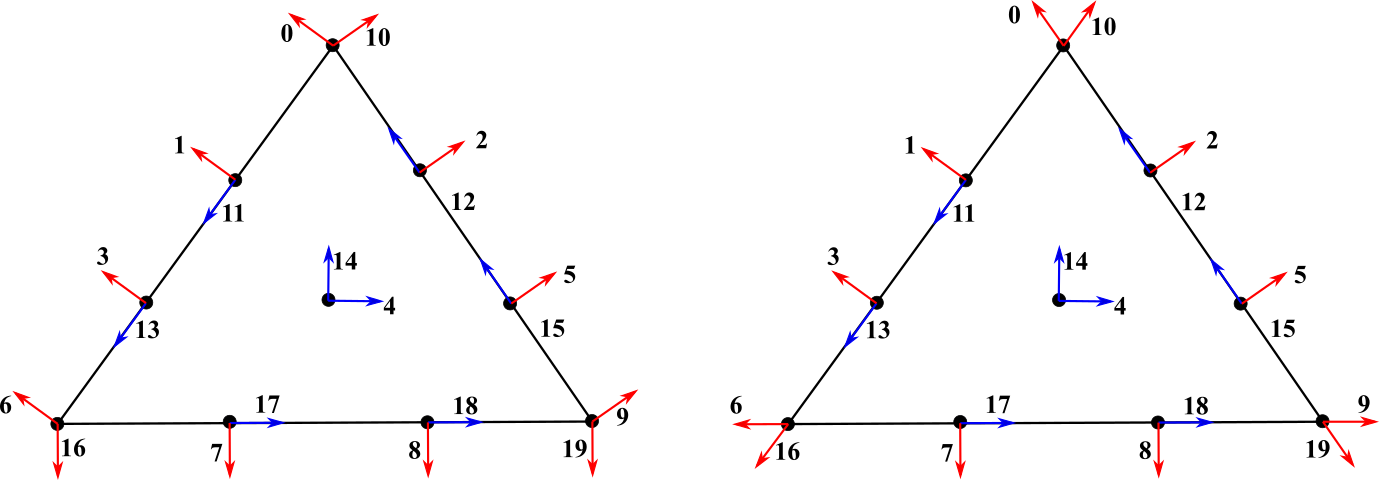
\includegraphics[width=0.8\textwidth]{figures/bdm2dfram.png}
%\caption{The left figure shows $\{\bs e_0, \bs e_1\}$ at each interpolation 
%point, the right figure shows $\{\hat{ \bs e}_0, \hat{ \bs e}_1\}$ 
%at each interpolation point.}
%\end{figure}
%
%Notice the dual basis on vertices is consistent with the general formulae \eqref{eq:dualnF} as $\bs n_{e,\texttt{v}}$ is the edge vector by definition.
%
%%\begin{lemma}[BDM element on triangle]\label{lemma:bdm2d}
%%   A polynomial function $\bs u \in \mathbb P_k^2(T)$ can be uniquely determined by the DoFs:
%%  $$
%%N^i_{\bs \alpha }(\bs u):=  \bs u(\bs x_{\bs \alpha}) \cdot \bs e_{\bs x}^i, \quad \bs x_{\bs \alpha} \in \mathcal X_{T}, i = 0, 1.
%%  $$
%%  The basis function of $k$th order BDM element space on $T$ can be 
%%  explicitly written as:
%%  $$
%%  \bs{\phi}_{\bs \alpha}^i(\bs x) = 
%%  \phi_{\bs\alpha}(\bs x) \hat{\bs e}^{\bs x_{\bs \alpha}}_i, \quad 
%%  \boldsymbol \alpha \in \mathbb T^2_k, i = 0, 1.
%%  $$
%%\end{lemma}
%
%%\begin{lemma}[BDM space on a triangulation]\label{lm:BDMTh}
%%Given a conforming triangulation $\mathcal T_h$, for each edge $e\in \Delta_1(\mathcal T_h)$, we choose a global normal vector $\bs n_e$ and the local tangential vector $\bs t_e(T)$. The following {\rm DoFs}
%%  \begin{align}
%%  \bs u(\bs x) \cdot \bs n_{e}, \quad & 
%%  \bs x \in \mathcal X_{e}, e \in \Delta_1(\mathcal T_h) \label{eq:bdm2d1}\\
%%  \bs u(\bs x)|_{T} \cdot \bs t_e(T), \quad & 
%%  \bs x \in \mathring{\mathcal X}_{e}, e \in \Delta_1(T), T \in 
%%\mathcal T_h\label{eq:bdm2d2}\\
%%  \bs u(\bs x) \cdot (1, 0), \quad 
%%  \bs u(\bs x) \cdot (0, 1), \quad & 
%%  \bs x \in \mathcal X_{\mathring{T}}, T \in \mathcal T_h
%%  \label{eq:bdm2d3}
%%  \end{align}
%%  define an $H(\div)$-conforming space 
%%  $V_h=\{\bs v_h\in H(\div, \Omega): \bs v_h|_T\in\mathbb P_k^2(T) \;\; 
%%  \forall~T\in\mathcal T_h\}$.
%%\end{lemma}
%%\begin{proof}
%%On each triagnle $T$, DoFs (\ref{eq:bdm2d1})-(\ref{eq:bdm2d3}) will determine a 
%%function in $\mathbb P_k(T, \mathbb R^2)$ by Lemma \ref{lemma:bdm2d}. For $e \in
%%\Delta_{1}(\mathcal T_h)$, DoF \eqref{eq:bdm2d1} restricted to
%%$e$ will determine the trace $\mathrm{tr^{div}}\bs u$ on $e$ 
%%independent of the triangles containing $e$ and thus the function is 
%%$H(\mathrm{div})$-conforming.
%%\end{proof}
%%
%%We call \eqref{eq:bdm2d1} as DoF on edge, \eqref{eq:bdm2d2} and 
%%\eqref{eq:bdm2d3} as DoF in cell. Notice that the tangential DoF \eqref{eq:bdm2d2} is local and thus double valued for an interior edge.
%
%\subsubsection{BDM element on tetrahedron meshes}
%%\begin{definition}
%Let $T$ be a tetrahedron,  for an interpolation point $\bs x \in \mathcal X_{T}$, 
%  we shall choose a frame $\{\bs e_{\boldsymbol x}^0, \bs e_{\bs x}^1, \bs e_{\bs x}^2\}$ 
%at $\bs x$ and its dual frame 
%$\{\hat {\bs e}_{\bs x}^0, \hat{\bs e}_{\bs x}^1, \hat{\bs e}_{\bs x}^2\}$ 
%as follows:
%\begin{enumerate}
%  \item For a vertex $\bs x \in \Delta_0(T)$, let adjacent edges of $\bs x$ be  
%    $e_0$, $e_1$, $e_2$, and the adjacent faces be   
%    $F_0$, $F_1$, $F_2$, satisfying $F_i \cap e_i = \bs x$, then
%  $$
%  \bs e_{\bs x}^0 = \bs n_{F_0}, \quad 
%  \bs e_{\bs x}^1 = \bs n_{F_1}, \quad 
%  \bs e_{\bs x}^2 = \bs n_{F_2},
%  $$
%  $$
%  \hat{\bs e}_{\bs x}^0 = \frac{\boldsymbol t_{e_0}}{\boldsymbol t_{e_0}
%    \cdot \boldsymbol n_{F_0}}, \quad 
%  \hat{\bs e}_{\bs x}^1 = \frac{\boldsymbol t_{e_1}}{\boldsymbol t_{e_1} 
%    \cdot \boldsymbol n_{F_1}}, \quad 
%  \hat{\bs e}_{\bs x}^2 = \frac{\boldsymbol t_{e_2}}{\boldsymbol t_{e_2} 
%    \cdot \boldsymbol n_{F_2}}.
%  $$ 
%  \item If $\bs x \in \mathcal X_{\mathring{e}}, e \in \Delta_1(T)$ 
%    with adjacent faces $F_0$, $F_1$, then
%  $$
%  \bs e_{\bs x}^0 = \bs n_{F_0}, \quad 
%  \bs e_{\bs x}^1 = \bs n_{F_1}, \quad	
%  \bs e_{\bs x}^2 = \bs t_{e},
%  $$  
%  $$
%  \hat{\bs e}_{\bs x}^0 = \frac{\bs n_{F_1}\times \bs t_e}{\bs n_{F_0} 
%    \cdot (\bs n_{F_1}\times \bs t_e)}, \quad 
%  \hat{\bs e}_{\bs x}^1 = \frac{\bs n_{F_0}\times \bs t_e}{\bs n_{F_1} 
%  \cdot (\bs n_{F_0}\times \bs t_e)}, \quad 
%  \hat{\bs e}_{\bs x}^2 = \bs t_{e}. 
%  $$  
%  \item If $\bs x \in \mathcal X_{\mathring{F}}$ with $F \in \Delta_2(T), e\in \partial F$, then
%  $$
%  \bs e_{\bs x}^0 = \bs n_{F}, \quad 	
%  \bs e_{\bs x}^1 = \bs t_{e} \times \bs n_F, \quad
%  \bs e_{\bs x}^2 = \bs t_{e},
%  $$ 
%  $$
%  \hat{\bs e}_{\bs x}^0 = \bs n_{F}, \quad 	
%  \hat{\bs e}_{\bs x}^1 = \bs t_{e} \times \bs n_F, \quad
%  \hat{\bs e}_{\bs x}^2 = \bs t_{e}.
%  $$
%  \item If $\bs x \in \mathcal X_{\mathring{T}}$, then
%  $$
%  \bs e_{\bs x}^0 = (1, 0, 0), \quad 
%  \bs e_{\bs x}^1 = \bs (0, 1, 0), \quad 
%  \bs e_{\bs x}^2 = \bs (0, 0, 1),
%  $$ 		
%  $$
%  \hat{\bs e}_{\bs x}^0 = (1, 0, 0), \quad 
%  \hat{\bs e}_{\bs x}^1 = \bs (0, 1, 0), \quad 
%  \hat{\bs e}_{\bs x}^2 = \bs (0, 0, 1).
%  $$ 		
%\end{enumerate}
%%\end{definition}
%
%The dual basis on edges is also consistent with \eqref{eq:dualnF} as $\bs n_{F_1}\times \bs t_e$ is $\bs n_{F_1,e}$. 
%
%\begin{figure}[htp]
%  \begin{minipage}[t]{0.48\textwidth}
%  \centering
%  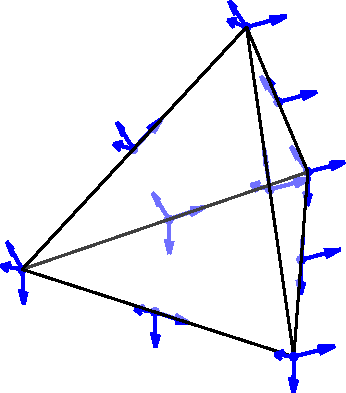
\includegraphics[width=0.5\textwidth]{figures/bdm_dof.pdf}
%  \end{minipage}
%  \begin{minipage}[t]{0.48\textwidth}
%  \centering
%  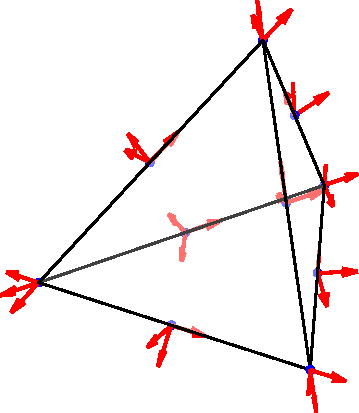
\includegraphics[width=0.5\textwidth]{figures/bdm_basis.pdf}
%  \end{minipage}
%  \caption{The left figure shows $\{\bs e_0, \bs e_1, \bs e_2\}$ at each 
%      interpolation point, the right figure shows 
%      $\{\hat{ \bs e}_0, \hat{ \bs e}_1, \hat{\bs e}_2\}$ 
%      at each interpolation point.}
%\end{figure}
%
%%\begin{lemma}[BDM element on a tetrahedron]\label{lemma:bdm3d}
%%  A polynomial function $\bs u \in \mathbb P_k^3(T)$ 
%%  can be uniquely determined by the DoFs:
%%  $$
%%N^i_{\bs \alpha }(\bs u):=  \bs u(\bs x_{\bs \alpha}) \cdot \bs e_{\bs x}^i, \quad \bs x_{\bs \alpha} \in \mathcal X_{T}, 
%%  i = 0, 1, 2.
%%  $$
%%  The basis function of $k$th order BDM element space on $T$ 
%%  can be explicitly written as:
%%  $$
%%  \label{eq:bdmbasis3d}
%%  \bs{\phi}_{\bs \alpha}^i(\bs x) = 
%%  \phi_{\bs\alpha}(\bs x) \hat{\bs e}^{\bs x_{\bs \alpha}}_i, 
%%  \quad \boldsymbol \alpha \in \mathbb T^3_k, i = 0, 1, 2.
%%  $$
%%\end{lemma}
%%
%%\begin{lemma}[BDM element on tetrahedron mesh]
%%Given a conforming triangulation $\mathcal T_h$, for each $F\in \Delta_2(\mathcal T_h)$, we choose a global normal vector $\bs n_F$ and two local tangential vectors $\bs t_F^0(T), \bs t_F^1(T)$. Also for each edge $e$, we choose a local tangential vector $\bs t_e(T)$.  The following {\rm DoFs}
%%  \begin{align}
%%    \bs u(\bs x) \cdot \bs n_F, \quad & 
%%    \bs x \in \mathcal X_{F}, F \in \Delta_2(\mathcal T_h), \label{eq:bdm3d1}\\
%%    \bs u(\bs x)|_{T} \cdot \bs t_{F}^0(T), \quad 
%%    \bs u(\bs x)|_{T} \cdot \bs t_{F}^1(T), \quad & 
%%    \bs x \in \mathring{\mathcal X}_{F}, F \in \Delta_2(T), T \in
%%\mathcal T_h, \label{eq:bdm3d2}\\
%%    \bs u(\bs x)|_{T} \cdot \bs t_{e}(T), \quad& 
%%    \bs x \in \mathring{\mathcal X}_{e}, \ e \in \Delta_1(T), T \in
%%\mathcal T_h, \label{eq:bdm3d3}\\
%%    \bs u(\bs x) \cdot \bs e_{\bs x}^i \quad & 
%%    \bs x \in \mathcal X_{\mathring{T}}, i=0,1,2, \ T \in
%%\mathcal T_h, \label{eq:bdm3d4}
%%  \end{align}
%%  define an $H(\div)$-conforming space $V_h=\{\bs v_h\in H(\div, \Omega): 
%%  \bs v_h|_{T}\in\mathbb P_k^3(T),\ \forall~T\in\mathcal T_h\}$.
%%\end{lemma}
%%\begin{proof}
%%On each tetrahedron $T$, DoFs (\ref{eq:bdm3d1})-(\ref{eq:bdm3d4}) will determine a 
%%function in $\mathbb P_k(T, \mathbb R^3)$ by Lemma \ref{lemma:bdm3d}. For 
%%$F \in \Delta_{2}(\mathcal T_h)$, DoF (\ref{eq:bdm3d1}) restricted to $F$ will determine the trace $\mathrm{tr^{div}}\bs u$ on $F$ 
%%independent of the tetrahedrons containing $F$ and thus the function is 
%%$H(\mathrm{div})$-conforming.
%%\end{proof}
%%We call \eqref{eq:bdm3d1} as DoFs on face, which is single valued, \eqref{eq:bdm3d2}, \eqref{eq:bdm3d3}, and \eqref{eq:bdm3d4} as DoFs in cell, which are multi-valued as the tangential vectors are local. 
%

%%%%%%%%%%%%%%%
\section{Geometric Decompositions of Edge Elements}\label{sec:edgefem}
In this section we present geometric decompositions of $H(\curl)$-conforming finite element space on an $n$-dimensional simplex. We first generalize the $\curl$ differential operator to $n$ dimensions and study its trace which motivates our decomposition. We then give an explicit basis dual to function values at interpolation points.

\subsection{Differential operator and its trace}
Denote by $\mathbb S$ and $\mathbb K$ the subspace of symmetric matrices and skew-symmetric matrices of $\mathbb R^{n\times n}$, respectively. For a smooth vector function $\boldsymbol{v}$, define
$$
\curl\boldsymbol{v}:=2\skw(\grad\boldsymbol{v}) = \grad\boldsymbol{v} - (\grad\boldsymbol{v})^{\intercal},
$$
which is a skew-symmetric matrix function. In two dimensions, for $\boldsymbol{v}=(v_1, v_2)^{\intercal}$,
$$
\curl\boldsymbol{v}=\begin{pmatrix}
0 & \partial_{x_2}v_1-\partial_{x_1}v_2 \\
\partial_{x_1}v_2-\partial_{x_2}v_1 & 0
\end{pmatrix}=\mskw(\rot\boldsymbol{v}),
$$
where
$
\mskw u:=\begin{pmatrix}
0 & -u \\
u & 0
\end{pmatrix}$ and $\rot\boldsymbol{v}:=\partial_{x_1}v_2-\partial_{x_2}v_1$.
In three dimensions, for $\boldsymbol{v}=(v_1, v_2, v_3)^{\intercal}$,
$$
\curl\boldsymbol{v}=\begin{pmatrix}
0 & \partial_{x_2}v_1-\partial_{x_1}v_2 & \partial_{x_3}v_1-\partial_{x_1}v_3 \\
\partial_{x_1}v_2-\partial_{x_2}v_1 & 0 & \partial_{x_3}v_2-\partial_{x_2}v_3 \\
\partial_{x_1}v_3-\partial_{x_3}v_1 & \partial_{x_2}v_3-\partial_{x_3}v_2 & 0 
\end{pmatrix}=\mskw(\nabla\times\boldsymbol{v}),
$$
where
$
\mskw \boldsymbol{u}:=\begin{pmatrix}
 0 & -u_3 & u_2 \\
u_3 & 0 & - u_1\\
-u_2 & u_1 & 0
\end{pmatrix}$ with $\boldsymbol{u}=(u_1, u_2, u_3)^{\intercal}$.
Hence we can identify $\curl\boldsymbol{v}$ as scalar $\rot\boldsymbol{v}$ in two dimensions, and vector $\nabla\times\boldsymbol{v}$ in three dimensions. In general, $\curl \bs u$ is understood as a skew-symmetric matrix. 


Define Sobolev space
\begin{equation*}
H(\curl,\Omega):=\{\boldsymbol{v}\in L^2(\Omega;\mathbb R^n): \curl\boldsymbol{v}\in L^2(\Omega;\mathbb K)\}.
\end{equation*}
Given a face $F\in \Delta_{n-1}(T)$, define the trace operator of $\curl$ as
$$
{\rm tr}_F^{\curl}\boldsymbol v=2\skw(\boldsymbol{v}\boldsymbol{n}_F^{\intercal})|_F = (\boldsymbol{v}\boldsymbol{n}_F^{\intercal} - \boldsymbol{n}_F\boldsymbol{v}^{\intercal})|_F.
$$
We define $\tr^{\curl}$ as a piecewise defined operator as $$(\tr^{\curl}\bs v) |_F = \tr^{\curl}_F\bs v, \quad F\in \Delta_{n-1}(T).$$

For a vector $\bs v\in \mathbb R^n$ and an $n-1$ dimensional face $F$, the tangential part of $\boldsymbol v$ on $F$ is
$$
\Pi_F\boldsymbol v := \boldsymbol v|_F - (\boldsymbol v|_F\cdot\boldsymbol n_F)\boldsymbol n_F = \sum_{i=1}^{n-1}(\boldsymbol v|_F\cdot\boldsymbol t_{i}^F)\boldsymbol t_{i}^F,
$$ 
where $\{ \bs t_{i}^F, i=1,\ldots, n-1 \}$ is an orthonormal basis of $F$. 
As we treat $\curl \bs v$ as a matrix, so is the trace ${\rm tr}_F^{\curl}\boldsymbol v$, while the tangential component of $\bs v$ is a vector. Their relation is given in the following lemma.

\begin{lemma}
For face $F\in \Delta_{n-1}(T)$, 
we have 
\begin{equation}\label{eq:tangentialtracetangentialpart}
{\rm tr}_F^{\curl}\boldsymbol v = 2\skw\big((\Pi_F\boldsymbol v)\boldsymbol{n}_F^{\intercal}\big), \quad \Pi_F\boldsymbol v = ({\rm tr}_F^{\curl}\boldsymbol v)\boldsymbol{n}_F.
\end{equation}
\end{lemma}
\begin{proof}
By the decomposition $\boldsymbol v|_F =\Pi_F\boldsymbol v + (\boldsymbol v|_F\cdot\boldsymbol n_F)\boldsymbol n_F$,
$$
{\rm tr}_F^{\curl}\boldsymbol v=2\skw\big((\Pi_F\boldsymbol v)\boldsymbol{n}_F^{\intercal} + (\boldsymbol v|_F\cdot\boldsymbol n_F)\boldsymbol n_F\boldsymbol{n}_F^{\intercal}\big) = 2\skw\big((\Pi_F\boldsymbol v)\boldsymbol{n}_F^{\intercal}\big),
$$
which implies the first identity.
Then by $\boldsymbol{n}_F^{\intercal}\boldsymbol{n}_F=1$ and $(\Pi_F\boldsymbol v)^{\intercal}\boldsymbol{n}_F=0$,
$$
({\rm tr}_F^{\curl}\boldsymbol v)\boldsymbol{n}_F=\big((\Pi_F\boldsymbol v)\boldsymbol{n}_F^{\intercal} - \boldsymbol{n}_F(\Pi_F\boldsymbol v)^{\intercal}\big)\boldsymbol{n}_F=\Pi_F\boldsymbol v,
$$
i.e. the second identity holds.
\end{proof}
Thanks to \eqref{eq:tangentialtracetangentialpart}, the vanishing tangential part $\Pi_F\boldsymbol v$ and the vanishing tangential trace $({\rm tr}_F^{\curl}\boldsymbol v)$ are equivalent.

\begin{lemma}
Let $\bs v \in L^2(\Omega;\mathbb R^n)$ and $\bs v|_T\in H^{1}(T;\mathbb S)$ for each $T\in \mathcal T_h$. Then $\bs v \in H(\curl,\Omega)$ if and only if $\,\Pi_F\boldsymbol v\mid_{T_1} = \Pi_F\boldsymbol v\mid_{T_2}\,$ for all interior face $F\in \Delta_{n-1}(\mathcal T_h)$, where $T_1$ and $T_2$ are two elements sharing $F$.
\end{lemma}
\begin{proof}
It is an immediate result of  Lemma 5.1 in~\cite{ArnoldFalkWinther2006} and \eqref{eq:tangentialtracetangentialpart}.
\end{proof}

\subsection{Polynomial bubble space}
Define the polynomial bubble space for the $\curl$ operator as
$$
\mathbb B_k(\curl, T) = \ker(\tr^{\curl})\cap \mathbb P_k^n(T).
$$
For Lagrange bubble space $\mathbb B_k^n(T)$, all components of the vector function vanish on $\partial T$ and consequently on all sub-simplex with dimension $\leq n-1$. For $\bs u \in \mathbb B_k(\curl, T)$, only the tangential component vanishes, which will imply $\bs u$ vanishes on sub-simplex with dimension $\leq n-2$. 

\begin{lemma}\label{lm:curlbubbleface}
For $\bs u\in \mathbb B_k(\curl, T)$, it holds $\bs u|_f=\bs0$ for all $f\in\Delta_{\ell}(T), 0\leq \ell\leq n-2$. Consequently $\mathbb B_k(\curl, T)\subset \mathbb B_k^n(T) \oplus\Oplus_{F\in \Delta_{n-1}(T)}  \mathbb B_k^{n}(F)$.
\end{lemma}
\begin{proof}
It suffices to consider a sub-simplex $f\in \Delta_{n-2}(T)$. Let $F_1, F_2\in\Delta_{n-1}(T)$ such that $f=F_1\cap F_2$. By $\tr_{F_i}^{\curl}\bs u=\bs0$ for $i=1,2$, we have $\Pi_{F_i}\bs u = 0$ and consequently
$$
(\bs u\cdot\bs t_i^f)|_f=0, \;\; (\bs u\cdot\bs n_{F_1}^f)|_f=(\bs u\cdot\bs n_{F_2}^f)|_f=0\quad \textrm{ for } i=1,\ldots, n-2,
$$
where $\bs n_{F_i}^f$ is a normal vector $f$ sitting on $F_i$. As $\spa \{\bs t_1^f, \ldots, \bs t_{n-2}^f, \bs n_{F_1}^f, \bs n_{F_2}^f \} = \mathbb R^n$, we acquire $\bs u|_f=\bs0$. By the property of face bubbles, we conclude $\bs u$ is a linear combination of element bubble and $n-1$ face bubbles. 
\end{proof}

Obviously $\mathbb B_k^n(T)\subset \mathbb B_k(\curl, T)$. As $\tr^{\curl}$ contains the tangential component only, the normal component $\mathbb B_k(F)\bs n_F$ is also a $\curl$ bubble. The following result says their sum is precisely all $\curl$ bubble polynomials.  
\begin{theorem}\label{thm:curlbubbletracespacedecomp}
For $k\geq 1$, it holds that
\begin{equation}\label{eq:curlbubbledecomp}
\mathbb B_k(\curl, T) =  \mathbb B_k^n(T) \oplus \Oplus_{F\in \Delta_{n-1}(T)} \mathbb B_k(F)\bs n_F,
\end{equation}
and
\begin{equation}\label{eq:trNrf}
{\rm tr}^{\curl} : \mathbb P_1^n(T)\oplus \Oplus_{\ell = 1}^{n-2}\Oplus_{f\in \Delta_{\ell}(T)} \mathbb B_k^n(f)\oplus \Oplus_{F\in \Delta_{n-1}(T)}  \mathbb B_k^{n-1}(F) \to  {\rm tr}^{\curl} \mathbb P_k^n(T)
\end{equation} 
% \begin{align}\label{eq:trNrf}
% {\rm tr} : &\Oplus_{i = 0}^{n}\lambda_{i}\mathbb P_{k - 1} ({\bs x}_i)\otimes \mathbb R^n \oplus \Oplus_{\ell = 1}^{n-1}\Oplus_{f\in \Delta_{\ell}(T)}  \mathscr{T}^f_k( T) \oplus \Oplus_{\ell = 0}^{n-2}\Oplus_{f\in \Delta_{\ell}(T)}  \mathscr{N}^f_k( T) \\
% &\to  {\rm tr} \mathbb P_k^n(T) \notag
% \end{align}
is a bijection.
\end{theorem}
\begin{proof}
It is obvious that
$$
\mathbb B_k^n(T) \oplus \Oplus_{F\in \Delta_{n-1}(T)} \mathbb B_k(F)\bs n_F \subseteq \mathbb B_{k}(\curl,T).
$$
Then apply the trace operator to the decomposition \eqref{eq:Pkvecdec}
% \begin{align}\label{eq:Pkvecdec}
% \mathbb P_k^n(T)&= \mathbb P_1^n(T)\oplus \Oplus_{\ell = 1}^n\Oplus_{f\in \Delta_{\ell}(T)} \mathbb B_{k}^n(f).
% \end{align}
 to conclude that 
%$$
%{\rm tr}^{\curl} \left( \mathbb P_1(T)\oplus \Oplus_{\ell = 1}^{n-2}\Oplus_{f\in \Delta_{\ell}(T)} \mathbb B_k^n(f)\oplus \Oplus_{F\in \Delta_{n-1}(T)}  \mathscr{T}^F_k( T) \right) =  {\rm tr}^{\curl} \mathbb P_k^n(T).
%$$ 
the map $\tr^{\curl}$ in~\eqref{eq:trNrf} is onto. 

Now we prove it is also injective. Take a function $\bs u\in  \mathbb P_1^n(T)\oplus \Oplus_{\ell = 1}^{n-2}\Oplus_{f\in \Delta_{\ell}(T)} \mathbb B_k^n(f)\oplus \Oplus_{F\in \Delta_{n-1}(T)}  \mathbb B_k^{n-1}(F)$ and $\tr^{\curl} \bs u =\bs 0$. By Lemma~\ref{lm:curlbubbleface}, we can assume $\bs u=\sum\limits_{F\in \Delta_{n-1}(T)}\bs u_k^F$ with $\bs u_k^F \in \mathbb B_k^{n-1}(F)$.
Take $F\in \Delta_{n-1}(T)$. We have $\bs u|_F=\bs u_k^F|_F\in \mathbb B_k^{n-1}(F)$. Hence $(\bs u_k^F\cdot\bs t)|_F=(\bs u\cdot\bs t)|_F=0$ for any $\bs t\in\mathscr T^F$, which results in $\bs u_k^F=\bs0$. Therefore $\bs u = \bs0$.  

% As $\bs u$ contains only normal component, DoF \eqref{eq:dofvectort} will be zero. For each $f\in \Delta_{\ell}(T)$, $\mathscr{N}^f = {\rm span}\{ \bs n_F, f\subset F\}$ and thus $\bs n_F\cdot \bs u = 0$ implies DoF \eqref{eq:dofvectorn} also vanishes. Therefore $\bs u = 0$. 
% Now we prove it is also injective. Take a function $\bs u\in \Oplus_{\ell = 0}^{n-1}\Oplus_{f\in \Delta_{\ell}(T)}  \mathscr{N}^f_k( T)$ and $\tr \bs u = 0$. As $\bs u$ contains only normal component, DoF \eqref{eq:dofvectort} will be zero. For each $f\in \Delta_{\ell}(T)$, $\mathscr{N}^f = {\rm span}\{ \bs n_F, f\subset F\}$ and thus $\bs n_F\cdot \bs u = 0$ implies DoF \eqref{eq:dofvectorn} also vanishes. Therefore $\bs u = 0$. 

Once we have proved the map $\tr$ in \eqref{eq:trNrf} is bijection, we conclude \eqref{eq:curlbubbledecomp} from the decomposition \eqref{eq:Pkvecdec}. 
%$ {\rm tr} \mathbb P_k\Lambda^{n-1}(T) = \sum_{\ell = 0}^{n-1}\sum_{f\in \Delta_{\ell}(T)} {\rm tr}  \left (\mathscr{N}^f_k( T)\right )$.
%\eqref{eq:trNrf}. \mnote{How to prove direct sum?}
% To prove ``=", we only need to count the dimensions. 
%Dimension count 
%$$
%\dim \mathbb B_k(\div, T)
%= \dim \mathbb P_k^n(T) - \dim {\rm tr}^{\div}(\mathbb P_k^n(T)). 
%$$
%We then do the dimension count which is straight forward in view of Fig. \ref{fig:Hdivdec}. 
\end{proof}

%\begin{corollary}
%The $\curl$ bubble space $\mathbb B_k(\curl, T)$ is uniquely determined by 
%\begin{align}
%\label{eq:dofcurlbubbleface}
%\int_F (\bs u\cdot \bs n_{F})\ p \dd s, &\quad p\in \mathbb P_{k - n}(F), F\in\partial T, \\ 
%\label{eq:dofcurlbubbleinterior}
%\int_T \bs u\cdot \bs q \dx, &\quad \bs q\in \mathbb P_{k-(n+1)}^n(T). 
%\end{align}
%\end{corollary}
%\begin{proof}
%Due to the decomposition \eqref{eq:curlbubbledecomp}, the number of \eqref{eq:dofcurlbubbleface} and \eqref{eq:dofcurlbubbleinterior} equals $\dim\mathbb B_k(\curl, T)$. Assume $\bs u\in \mathbb B_k(\curl, T)$, and \eqref{eq:dofcurlbubbleface}-\eqref{eq:dofcurlbubbleinterior} vanish. By the decomposition \eqref{eq:curlbubbledecomp}, $(\bs u\cdot \bs n_{F})|_F\in \mathbb B_k(F)$, then the vanishing \eqref{eq:dofcurlbubbleface} implies $(\bs u\cdot \bs n_{F})|_F=0$. Thus $\bs u\in \mathbb B_k^n(T)$, which together with the vanishing~\eqref{eq:dofcurlbubbleinterior} yields $\bs u=\bs0$. 
%\end{proof}

%
%Define $\mathbb B_k(F) =  b_f\mathbb P_{k - (\ell +1)} (f)$ for $f\in\Delta_{\ell}(T)$ and $\ell=0,\ldots, n$, and

We will use $\curl_f$ to denote the $\curl$ operator restricted to a sub-simplex $f$ with $\dim f \geq 1$. For $f\in\Delta_{\ell}(T), \ell=2,\ldots, n-1$, by applying Theorem~\ref{thm:curlbubbletracespacedecomp} to $f$, we have
\begin{equation}\label{eq:curlfbubble}
\mathbb B_k(\curl_f, f) = \mathbb B_{k}^{\ell}(f) \oplus \Oplus_{e\in \partial f}\mathbb B_{k}( e) \boldsymbol{n}_{f}^e.
\end{equation}
% where $\bs n_{f}^e$ is a normal vector of $e$ but parallel to $f$. 
%Here $\curl_f$ operator is the exterior derivative of an $1$-form on $f$. 
Notice that the $\curl_f$-bubble function is defined for $\ell \geq 2$ not including edges. 
Indeed, for an edge $e$ and a vertex ${\bs x}$ of $e$, $\boldsymbol{n}_{e}^{\bs x}$ is $\boldsymbol{t}_{e}$ if $\bs x$ is the ending vertex of $e$ and $-\boldsymbol{t}_{e}$ otherwise. Then for $\ell = 1$
\begin{equation}\label{eq:curlebubble}
\mathbb B_{k}( e) \bs t_e \oplus \Oplus_{{\bs x}\in \partial e} {\rm span}\{\lambda_{\bs x} \boldsymbol{n}_{e}^{\bs x}\} = \mathbb P_{k}(e)\bs t_e.
\end{equation}
which is the full polynomial not vanishing on $\partial e$. 
%Indeed for one dimensional edge $e\in \Delta_1(T)$
%$$
%\mathbb B_k(\curl; e) = \mathbb B_k(\grad; e)\bs t^e = \mathbb B_k(e) \bs t^e.  
%$$

\subsection{Geometric decompositions}
For $e\in\Delta_{\ell}(T)$, we choose the basis $\{\bs n_{f}^e: f = e+i, i\in e^*\}$ for $\mathscr{N}^e$ and a basis $\{\bs t_i^e,  i=1,\ldots,\ell\}$ for $\mathscr{T}^e$. So we have the following geometric decompositions of $\mathbb P_k^n(T) $. 
\begin{theorem}
For $k\geq 1$, we have
\begin{align}
\label{eq:curlpolynomialdecomp}
\mathbb P_k^n(T) &= \mathbb P_1^n(T) \oplus \Oplus_{\ell=1}^n \Oplus_{e\in\Delta_{\ell}(T)}\mathbb B_k(e)\otimes \spa\{\bs t_i^e\}_{i=1}^{\ell} \oplus \mathbb B_k(e)\otimes \spa\{\bs n_{e+i}^e, i\in e^*\},\\
%\mathbb P_k^n(T) &= \mathbb P_1^n(T) \oplus \Oplus_{e\in\Delta_{1}(T)}\mathbb B_k(e)\bs t_e \oplus \Oplus_{\ell=2}^n\Oplus_{f\in\Delta_{\ell}(T)}\mathbb B_k(\curl_f, f),\\
\label{eq:curlpolynomialdecomp2}
\mathbb P_k^n(T) &= \Oplus_{e\in \Delta_1(T)}\mathbb P_k(e)\bs t_e \oplus \Oplus_{\ell=2}^n\Oplus_{f\in\Delta_{\ell}(T)}\mathbb B_k(\curl_f, f).
\end{align}
\end{theorem}
\begin{proof}
Decomposition \eqref{eq:curlpolynomialdecomp} is the component form of decomposition \eqref{eq:Pkvecdec}. We can write $\mathbb B_k(e)\otimes \spa\{\bs n_{e+i}^e, i\in e^*\} = \Oplus_{f\in \Delta_{\ell+1}(T),e\subseteq f}\mathbb B_k( e)\boldsymbol{n}_{f}^e.$
%For $e\in\Delta_{\ell-1}(T)$, the face normal vectors $\{\bs n_{f}^e: f\in \Delta_{\ell}(T), e\subseteq f\}$ form a basis of $\mathscr{N}^e$. So we have
%$$
%\mathbb B_k( e) \otimes \mathscr{N}^e =\Oplus_{f\in \Delta_{\ell}(T), e\subseteq f}\mathbb B_k( e)\boldsymbol{n}_{f}^e.
%$$
Then in the summation \eqref{eq:curlpolynomialdecomp}, we shift the normal component one level up and switch the sum of $e$ and $f$:
% and use \eqref{eq:curlfbubble} to get the decomposition \eqref{eq:curlpolynomialdecomp}. 
% Then we write
\begin{align*}
&\Oplus_{\ell = 1}^n\Oplus_{e\in \Delta_{\ell}(T)} \big [ \mathbb B_{k}^{\ell}(e)\Oplus_{f\in \Delta_{\ell+1}(T),e\subseteq f}\mathbb B_k( e)\boldsymbol{n}_{f}^e \big ]\\
=&\Oplus_{e\in\Delta_{1}(T)}\mathbb B_k(e)\bs t_e \oplus \Oplus_{\ell=2}^n\Oplus_{f\in\Delta_{\ell}(T)}\big [\mathbb B_{k}^{\ell}(f) \Oplus_{e\subseteq \partial f}\mathbb B_k( e)\boldsymbol{n}_{f}^e \big ].
\end{align*}
Then by the characterization \eqref{eq:curlfbubble} of $\mathbb B_k(\curl_f, f)$ and \eqref{eq:curlebubble}, we get the decomposition \eqref{eq:curlpolynomialdecomp2}.
%
% We then distribute the $n$-component of vector function value at a vertex to the $n$ edges connected to this vertex. For a vertex $\bs x$ of $T$, there are $n$ edges of $T$ containing this vertex. We use $n$ edge vectors as a basis of $\mathbb R^n$ and thus
% $$
% \mathbb P_1^n(T) \oplus \Oplus_{e\in \Delta_1(T)}\mathbb B_k( e)\bs t_e = \Oplus_{e\in \Delta_1(T)} \left (\mathbb P_1(e)\bs t_e \oplus \mathbb B_k( e)\bs t_e\right) = \Oplus_{e\in \Delta_1(T)}\mathbb P_k(e)\bs t_e.
% $$
% %It is easy to see that $\mathbb P_k(e)=\mathbb P_1(e)\oplus \mathbb B_k( e)$. 
% Thus \eqref{eq:curlpolynomialdecomp2} holds.
\end{proof}
Decomposition \eqref{eq:curlpolynomialdecomp2} is the counterpart of \eqref{eq:Lagdecbubble} for Lagrange element. 
%In decomposition~\eqref{eq:curlpolynomialdecomp2}, the linear vector polynomial $\mathbb P_1^n(T)$ is redistributed to edges and the second kind N\'ed\'elec edge element~\cite{Nedelec1986} can be derived. 

\subsection{Tangential-Normal decomposition of the second family of edge elements}
Recall that for $e\in\Delta_{\ell-1}(T)$, the basis 
$\{\bs n_{f}^e: f\in \Delta_{\ell}(T), e\subseteq f\}$ of $\mathscr{N}^e$ is dual to the basis $\{\bs n_{F}: F\in \Delta_{n-1}(T), e\subseteq F\}$; see Lemma \ref{lm:dualnormal}.  

\begin{theorem}\label{thm:NedelecTNdecomp}
Take $\mathbb P_k^n(T)$ as the shape function space.
% Given an $e\in \Delta_{\ell-1}(T)$, we choose $\{\bs n_{f}^e, e\subseteq f\in\Delta_{\ell}(T)\}$ as the basis for the normal plane $\mathscr N^e$ and a basis $\{\bs t_i^e\}$ of $\mathscr T^e$. Then the DoFs%, for $\ell = 1,\ldots, n$, 
%\begin{subequations}
%\label{eq:dofveccurl}
%\begin{align}
%\label{eq:dofvectortcurl}
%\int_e (\bs u\cdot \bs t_i^e)\ p \dd s,& \quad i=1,\ldots, \ell-1, p\in \mathbb P_{k - \ell} (e), e\in \Delta_{\ell-1}(T), \ell = 2,\ldots, n,\\
%\label{eq:dofvectorncurl}
%\int_e (\bs u\cdot \bs n_{f}^e)\ p \dd s, &\quad f\in\Delta_{\ell}(T), e\subseteq f, p\in \mathbb P_{k - \ell} (e), e\in \Delta_{\ell-1}(T), \ell = 1,\ldots, n,\\ 
%\label{eq:dofvectorElementcurl}
%\int_T \bs u\cdot \bs q \dx, &\quad \bs q\in \mathbb B_k^n(T) 
%\end{align}
%\end{subequations}
%are equivalent to the second-kind N\'ed\'elec element
Then it is determined by the following DoFs
\begin{subequations}\label{eq:dofNedelec}
\begin{align}
\label{eq:dofvectoredgecurl}
\int_e \bs u\cdot \bs t\ p \dd s,& \quad p\in \mathbb P_{k} (e), e\in \Delta_1(T),\\
\label{eq:dofvectorfacecurl}
\int_f \bs u\cdot \bs p \dd s,& \quad \bs p\in \mathbb B_k(\curl_f, f),f\in\Delta_{\ell}(T), \ell=2,\ldots, n
%, \\
%\label{eq:bubbleDoFcurl}
%\int_T \bs u \cdot \bs p \dx, &\quad \bs p\in \mathbb B_k(\curl, T). 
\end{align}
\end{subequations}
\end{theorem}
\begin{proof}
%The unisolvence of DoFs \eqref{eq:dofveccurl} for $\mathbb P_k^n(T)$ follows from the geometric decomposition \eqref{eq:curlpolynomialdecomp2} and \eqref{eq:curlfbubble}.
%% Corollary~\ref{lm:vecLdec} by switching the normal basis $\{\bs n_1^e, \dots, \bs n_{n-\ell+1}^e\}$ to $\{\bs n_{f}^e, e\subseteq f\in\Delta_{\ell}(T)\}$.
%
%By rearranging $e$ and $f$, DoFs \eqref{eq:dofveccurl} can be rewritten as
Based on the decomposition \eqref{eq:curlpolynomialdecomp}, the shape function $\mathbb P_k^n(T)$ is determined by the following DoFs
\begin{subequations}
\label{eq:dofveccurlf}
\begin{align}
\label{eq:dofvectortedgecurlf}
\int_e \bs u\cdot \bs t\ p \dd s,& \quad p\in \mathbb P_{k} (e), e\in\Delta_1(T),\\
\label{eq:dofvectortcurlf}
\int_f (\bs u\cdot \bs t_i^f)\ p \dd s,& \quad p\in \mathbb P_{k - (\ell +1)} (f), i=1,\ldots, \ell, \\
\label{eq:dofvectorncurlf}
\int_e (\bs u\cdot \bs n_{f}^e)\ p \dd s, &\quad p\in \mathbb P_{k - \ell} (e), e\in\partial f 
\end{align}
\end{subequations}
for $f\in \Delta_{\ell}(T), \ell = 2,\ldots, n$.
By \eqref{eq:curlbubbledecomp} and \eqref{eq:curlfbubble},  DoFs \eqref{eq:dofveccurlf} are equivalent to DoFs \eqref{eq:dofNedelec}.
\end{proof}


%For $e\in \Delta_{\ell-1}(T)$, we redistribute the normal DoFs $\int_e (\bs u\cdot \bs n_{j}^e)\ p \dd s$ on $e$ with $j=1,\ldots, n-\ell+1$ and $p\in \mathbb P_{k - \ell} (e)$ to the tangential part \eqref{eq:dofvectorncurl} of $f$ for $e\subseteq f\in\Delta_{\ell}(T)$.

\begin{remark}\rm
 The DoFs of the second kind N\'ed\'elec edge element in~\cite{Nedelec1986,ArnoldFalkWinther2006} are
\begin{align*}
\int_e \bs u\cdot \bs t\ p \dd s,& \quad p\in \mathbb P_{k} (e), e\in \Delta_1(T), \\
\int_f \bs u\cdot \bs p \dd s,& \quad \bs p\in \mathbb P_{k-\ell}^{\ell}(f)+(\Pi_f\bs x)\mathbb P_{k-\ell}(f), f\in\Delta_{\ell}(T), \ell=2,\ldots, n. 
%\\
%\int_T \bs u \cdot \bs p \dx, &\quad \bs p\in \mathbb P_{k-n}^n(T)+\bs x\mathbb P_{k-n}(T). 
\end{align*} 
There is an isomorphism between $\mathbb P_{k-\ell}^{\ell}(f)+(\Pi_f\bs x)\mathbb P_{k-\ell}(f)$ and $\mathbb B_k(\curl_f, f)$ for $f\in\Delta_{\ell}(T)$ with $\ell=2, \ldots, n$, that is $\mathbb B_k(\curl_f, f)$ is uniquely determined by DoF 
\begin{equation*}
\int_f \bs u\cdot \bs p \dd s, \quad \bs p\in \mathbb P_{k-\ell}^{\ell}(f)+(\Pi_f\bs x)\mathbb P_{k-\ell}(f),
\end{equation*}
whose proof can be found in Lemma 4.7 in~\cite{ArnoldFalkWinther2006}.
$\qed$
\end{remark}

Given an $e\in \Delta_{\ell-1}(T_h)$, we choose a global $\{\bs n_{f}^e, e\subseteq f\in\Delta_{\ell}(T_h)\}$ as the basis for the normal plane $\mathscr N^e$ and a global basis $\{\bs t_i^e\}$ of $\mathscr T^e$. 
 Define the global finite element space
\begin{align*}
V_h^{\curl}:=\{\bs u\in L^2(\Omega;\mathbb R^n): &\bs u|_T\in\mathbb P_k(T; \mathbb R^n) \textrm{ for each } T\in\mathcal T_h, \\
% &\textrm{ all the DoFs \eqref{eq:dofvectortcurl} across $e\in\Delta_{\ell}(\mathcal T_h)$ are single-valued for  $\ell=1, \ldots, n-1$}, \\
 &\textrm{ all the DoFs \eqref{eq:dofNedelec} are single-valued}\}.
\end{align*}
%Since DoFs \eqref{eq:dofveccurl} are equivalent to DoFs \eqref{eq:dofNedelec}, we have $V_h^{\curl}\subset H(\curl,\Omega)$.

\begin{lemma}
We have $V_h^{\curl}\subset H(\curl,\Omega)$.
\end{lemma}
\begin{proof}
For an $F\in\Delta_{n-1}(T)$, DoFs \eqref{eq:dofveccurlf} related to $\Pi_F\bs u$ are
\begin{align*}
\int_e (\Pi_F\bs u\cdot \bs t_i^e)\ p \dd s,& \quad i=1,\ldots, \ell-1, p\in \mathbb P_{k - \ell} (e), e\in \Delta_{\ell-1}(F), \ell = 2,\ldots, n,\\
\int_e (\Pi_F\bs u\cdot \bs n_{f}^e)\ p \dd s, &\quad f\in\Delta_{\ell}(F), e\subseteq f, p\in \mathbb P_{k - \ell} (e), e\in \Delta_{\ell-1}(F), \ell = 1,\ldots, n-1,
\end{align*}
thanks to DoFs \eqref{eq:dofveccurlf}, which uniquely determine $\Pi_F\bs u$.
\end{proof}


\subsection{A nodal basis for the second-kind N\'ed\'elec edge element}

%For an interpolation point $\bs x\in e\in \Delta_{\ell}(T)$, we collect the above $t-n$ basis together and write as $\{\bs e_i^{f}, i=0,\ldots, n-1\} = \{ \bs t_i^f, i=1,\ldots, \ell,  \; \bs n_{f}^e,  f= e+i, i\in e^*\}$ and its dual basis $\{\hat{\bs e}_i^{f}, i=0,\ldots, n-1\} = \{ \hat{\bs t}_i^f, i=1,\ldots, \ell, \bs n_{F_i}/ (\bs n_{F_i}\cdot \bs n^e_{e+i}), i\in e^*\}$.
% For $\bs x_{\alpha} \in \mathcal X_{\mathring{f}}, f \in \Delta_{\ell}(T)$, by Corollary \ref{lem:basisfunctions}, the basis related to $\bs x_{\alpha}$ are
% $$
% \phi_{\bs\alpha}(\bs x)\bs t_i^f, i=1,\ldots, \ell; \quad
% \frac{1}{\bs n_{f+i}^f\cdot\bs n_{F_i}}\phi_{\bs\alpha}(\bs x)\bs n_{f+i}^f,  i\in f^*. 
% $$

By Corollary \ref{cor:basisfunctions}, we obtain a nodal basis for the second-kind N\'ed\'elec edge element.

\begin{theorem}
For each $e\in \Delta_{\ell}(T), \ell = 0,1,\ldots, n$, we choose $\{\bs e_i^{e}, i=0,\ldots, n-1\} = \{ \bs t_i^e, i=1,\ldots, \ell, \; \; \; \bs n_{f}^e,  f= e+i, i\in e^*\}$ and its dual basis $\{\hat{\bs e}_i^{e}, i=0,\ldots, n-1\} = \{ \hat{\bs t}_i^e, i=1,\ldots, \ell, \bs n_{F_i}/ (\bs n_{F_i}\cdot \bs n^e_{e+i}), i\in e^*\}$.
A basis function of the $k$-th order second kind N\'ed\'elec edge element space on $T$ is:
$$
\{\phi_{\bs\alpha}(\bs x)\hat{\bs e}^e_{i},  i=0,1,\ldots, n-1, \; \;  \alpha \in \mathbb T_k^{\ell}(\mathring{e})\}_{e \in \Delta_{\ell}(T), \ell =0,1,\ldots, n},
$$
with the DoFs at the interpolation points defined as:
\begin{align}\label{edgenodalDoFs}
\{u(\boldsymbol x_{\alpha})\bs e^e_i,  i=0,1,\ldots, n-1, \; \;  \boldsymbol x_{\alpha} \in \mathcal X_{\mathring{e}} \}_{e \in \Delta_{\ell}(T), \ell =0,1,\ldots, n}.
\end{align}
\end{theorem}

Notice that the basis $\{\bs t^e_i\}$ depends only on $e$ and $\bs n_{f}^e$ depends on $e$ and $f$ but independent $T$. By asking the corresponding DoFs single valued, we obtain the tangential continuity. 
%
We can define the edge finite element space as
\begin{align*}
V_h^{\curl}:=\{&\bs u\in L^2(\Omega;\mathbb R^n): \bs u|_T\in\mathbb P_k(T; \mathbb R^n) \textrm{ for each } T\in\mathcal T_h, \textrm{ the DoFs } u(\boldsymbol x_{\alpha})\bs t^e_i, u(\boldsymbol x_{\alpha})\bs n^e_f \\
% &\textrm{ all the DoFs \eqref{eq:dofvectortcurl} across $e\in\Delta_{\ell}(\mathcal T_h)$ are single-valued for  $\ell=1, \ldots, n-1$}, \\
 &\text{ in \eqref{edgenodalDoFs} are single-valued across all $e$ and $f$ with $\dim e, \dim f \leq n-1$}\}.
\end{align*}

%\begin{theorem}\label{th:Nedelecelement}
%% Take $\mathbb P_k^n(T)$ as the shape function space.
% Given an $e\in \Delta_{\ell-1}(T)$, we choose $\{\bs n_{f}^e, e\subseteq f\in\Delta_{\ell}(T)\}$ as the basis for the normal plane $\mathscr N^e$ and a basis $\{\bs t_i^e\}$ of $\mathscr T^e$. Then the DoFs%, for $\ell = 1,\ldots, n$, 
%\begin{subequations}chen1009

%\label{eq:dofveccurlPoint}
%\begin{align}
%\label{eq:dofvectortcurlPoint}
%\bs u(\bs x)\cdot \bs t_i^e,& \quad \bs x \in \mathcal X_{\mathring{e}}, i=1,\ldots, \ell-1, e\in \Delta_{\ell-1}(T), \ell = 2,\ldots, n,\\
%\label{eq:dofvectorncurlPoint}
%\bs u(\bs x)\cdot \bs n_{f}^e, &\quad \bs x \in \mathcal X_{\mathring{e}}, f\in\Delta_{\ell}(T), e\subseteq f, e\in \Delta_{\ell-1}(T), \ell = 1,\ldots, n,\\ 
%\label{eq:dofvectorElementcurlPoint}
%\bs u(\bs x), &\quad \bs x \in \mathcal X_{\mathring{T}}
%\end{align}
%\end{subequations}
%are uni-solvent for space $\mathbb P_k^n(T)$.
%And $V_h^{\curl}$ is same as 
%the global finite element space
%\begin{align*}
%&\{\bs u\in L^2(\Omega;\mathbb R^n): \bs u|_T\in\mathbb P_k(T; \mathbb R^n) \textrm{ for each } T\in\mathcal T_h, \\
% &\textrm{ all the DoFs \eqref{eq:dofvectortcurlPoint} across $e\in\Delta_{\ell}(\mathcal T_h)$ are single-valued for  $\ell=1, \ldots, n-1$}, \\
% &\textrm{ all the DoFs \eqref{eq:dofvectorncurlPoint} across $f\in\Delta_{\ell}(\mathcal T_h)$ are single-valued for  $\ell=1, \ldots, n-1$}\}.
%\end{align*}
%\end{theorem}
%\begin{proof}
%Apply Theorem~\ref{thm:NedelecTNdecomp} and the nodal DoFs (simplicial lattices) of Lagrange element.
%\end{proof}

%We call \eqref{eq:dofvectortcurlPoint} with $e\in\Delta_{\ell}(\mathcal T_h)$ and \eqref{eq:dofvectorncurlPoint} with $f\in\Delta_{\ell}(\mathcal T_h)$ as DoFs on $\ell$-dimensional faces,
%\eqref{eq:dofvectorncurlPoint} with $\ell=n$ and \eqref{eq:dofvectorElementcurlPoint} as DoFs in cell.

%By Lemma~\ref{lm:dualnormal}, the dual basis of $\{\bs n_{f+i}^f\}_{i\in f^*}$ are $\{\frac{1}{\bs n_{f+i}^f\cdot\bs n_{F_i}}\bs n_{F_i}\}_{i\in f^*}$. 
%For $\bs x_{\alpha} \in \mathcal X_{\mathring{f}}, f \in \Delta_{\ell}(T)$, by Corollary \ref{lem:basisfunctions}, the basis related to $\bs x_{\alpha}$ is
%$$
%\{\phi_{\bs\alpha}(\bs x)\bs t_i^f, i=1,\ldots, \ell; \quad
%\phi_{\bs\alpha}(\bs x)\bs n_{F_i}/ (\bs n_{F_i}\cdot \bs n^f_{f+i}),  i\in f^*\}.
%$$
%We present explicit formulae in two and three dimensions. 

\subsubsection{2D basis on triangular meshes}
%\begin{definition}
Let $T$ be a triangle, for lattice point $\boldsymbol{x}$ located in different sub-simplices, %on vertices, edges, and interior,  
we shall choose different frame $\{\bs e_{\boldsymbol x}^0, \bs e_{\bs x}^1\}$ 
at $\bs x$ and its dual frame 
$\{\hat {\bs e}_{\bs x}^0, \hat{\bs e}_{\bs x}^1\}$ 
as follows:
\begin{enumerate}
  \item If $\bs x \in \Delta_0(T)$, assume the two adjacent edges are $e_0$ 
    and $e_1$, then
  $$
  \bs e_{\bs x}^0 = \bs t_{e_0}, \quad 
  \bs e_{\bs x}^1 = \bs t_{e_1}, \quad
  \hat{\bs e}_{\bs x}^0 = \frac{\boldsymbol n_{e_1}}{\boldsymbol n_{e_1} 
  \cdot \boldsymbol t_{e_0}},
   \quad 
  \hat{\bs e}_{\bs x}^1 = \frac{\boldsymbol n_{e_0}}{\boldsymbol n_{e_0} 
  \cdot \boldsymbol t_{e_1}}.
  $$
  \item If $\bs x \in \mathcal X_{\mathring{e}}, e \in \Delta_1(T)$, 
    then
  $$
  \bs e_{\bs x}^0 = \bs t_{e}, \quad \bs e_{\bs x}^1 = \bs n_{e}, \quad	
  \hat{\bs e}_{\bs x}^0 = \bs t_{e}, \quad \hat{\bs e}_{\bs x}^1 = \bs n_{e}.	
  $$  
  \item If $\bs x \in \mathcal X_{\mathring{T}}$, then
  $$
  \bs e_{\bs x}^0 = (1, 0), \quad \bs e_{\bs x}^1 = \bs (0, 1), \quad
  \hat{\bs e}_{\bs x}^0 = (1, 0), \quad \hat{\bs e}_{\bs x}^1 = \bs (0, 1).
  $$		
\end{enumerate}
%\end{definition}

\begin{figure}[htp]
\centering
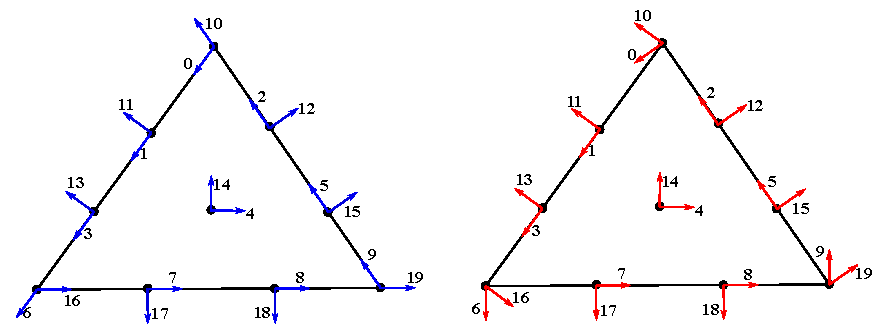
\includegraphics[width=0.8\textwidth]{figures/nedelec.pdf}
\caption{The left figure shows $\{\bs e_0, \bs e_1\}$ at each interpolation 
point, the right figure shows $\{\hat{ \bs e}_0, \hat{ \bs e}_1\}$ 
at each interpolation point.}
\end{figure}

\subsubsection{3D basis on tetrahedron meshes}
%\begin{definition}
  Let $T$ be a tetrahedron, for any $\bs x \in \mathcal X_{T}$, 
  define a frame $\{\bs e_{\boldsymbol x}^0, \bs e_{\bs x}^1, \bs e_{\bs x}^2\}$ 
  at $\bs x$ and its dual frame 
  $\{\hat {\bs e}_{\bs x}^0, \hat{\bs e}_{\bs x}^1, \hat{\bs e}_{\bs x}^2\}$ 
  as follows:
\begin{enumerate}
  \item If $\bs x \in \Delta_0(T)$ and adjacent edges of $\bs x$ are 
    $e_0$, $e_1$, $e_2$, adjacent faces of $\bs x$ are 
    $f_0$, $f_1$, $f_2$, then
  $$
  \bs e_{\bs x}^0 = \bs t_{e_0}, \quad 
  \bs e_{\bs x}^1 = \bs t_{e_1}, \quad 
  \bs e_{\bs x}^2 = \bs t_{e_2},
  $$
  $$
  \hat{\bs e}_{\bs x}^0 = \frac{\boldsymbol n_{f_0}}{\boldsymbol n_{f_0} 
    \cdot \boldsymbol t_{e_0}}, \quad 
  \hat{\bs e}_{\bs x}^1 = \frac{\boldsymbol n_{f_1}}{\boldsymbol n_{f_1} 
    \cdot \boldsymbol t_{e_1}}, \quad 
  \hat{\bs e}_{\bs x}^2 = \frac{\boldsymbol n_{f_2}}{\boldsymbol n_{f_2} 
    \cdot \boldsymbol t_{e_2}}.
  $$
  \item If $\bs x \in \mathcal X_{\mathring{e}}, e \in \Delta_1(T)$ 
    and adjacent faces are $f_0$, $f_1$ then
  $$
  \bs e_{\bs x}^0 = \bs t_{e}, \quad 
  \bs e_{\bs x}^1 = \bs n_{f_0}\times \bs t_{e}, \quad 
  \bs e_{\bs x}^2 = \bs n_{f_1}\times \bs t_{e},	
  $$ 
  $$
  \hat{\bs e}_{\bs x}^0 = \bs t_{e}, \quad 
  \hat{\bs e}_{\bs x}^1 = \frac{\boldsymbol n_{f_1}}{\boldsymbol n_{f_1} 
    \cdot (\boldsymbol n_{f_0}\times \boldsymbol t_e)}, \quad	
  \hat{\bs e}_{\bs x}^2 = \frac{\boldsymbol n_{f_0}}{\boldsymbol n_{f_0} 
    \cdot (\boldsymbol n_{f_1}\times \boldsymbol t_e)}.
  $$
  \item If $\bs x \in \mathcal X_{\mathring{f}}, f \in \Delta_2(T)$, 
    the first edge of $f$ is $e$, then
  $$
  \bs e_{\bs x}^0 = \bs t_{e}, \quad 
  \bs e_{\bs x}^1 = \bs t_{e} \times \bs n_f, \quad
  \bs e_{\bs x}^2 = \bs n_{f},
  $$
  $$
  \hat{\bs e}_{\bs x}^0 = \bs t_{e}, \quad 
  \hat{\bs e}_{\bs x}^1 = \bs t_{e} \times \bs n_f, \quad
  \hat{\bs e}_{\bs x}^2 = \bs n_{f}.	
  $$
  \item If $\bs x \in \mathcal X_{\mathring{T}}$, then
  $$
  \bs e_{\bs x}^0 = (1, 0, 0), \quad 
  \bs e_{\bs x}^1 = \bs (0, 1, 0), \quad 
  \bs e_{\bs x}^2 = \bs (0, 0, 1),
  $$
  $$
  \hat{\bs e}_{\bs x}^0 = (1, 0, 0), \quad 
  \hat{\bs e}_{\bs x}^1 = \bs (0, 1, 0), \quad 
  \hat{\bs e}_{\bs x}^2 = \bs (0, 0, 1).
  $$
\end{enumerate}
%\end{definition}

\begin{figure}[htp]
  \begin{minipage}[t]{0.48\textwidth}
  \centering
  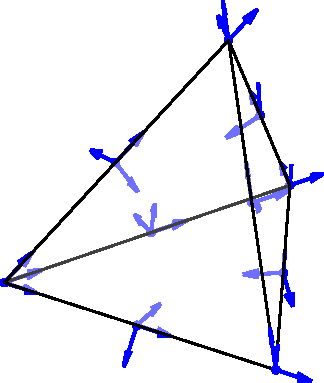
\includegraphics[width=0.5\textwidth]{figures/nedelec_dof.pdf}
  \end{minipage}
  \begin{minipage}[t]{0.48\textwidth}
  \centering
  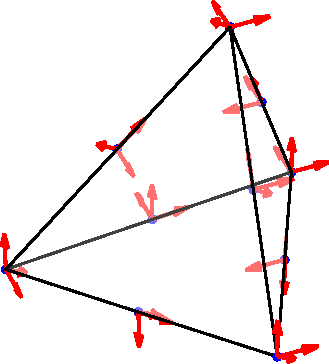
\includegraphics[width=0.5\textwidth]{figures/nedelec_basis.pdf}
  \end{minipage}
  \caption{The left figure shows $\{\bs e_0, \bs e_1, \bs e_2\}$ at each 
      interpolation point, the right figure shows 
      $\{\hat{ \bs e}_0, \hat{ \bs e}_1, \hat{\bs e}_2\}$ 
      at each interpolation point.}
\end{figure}

% \subsection{Geometric decomposition of first family of N\'ed\'elec element}
% The shape function space of the first family of N\'ed\'elec element is 
% \begin{equation*}
% \mathbb P_{k}^+(\curl, T):=\{\boldsymbol{v}\in\mathbb P_{k+1}^n(T): \boldsymbol{v}\cdot\boldsymbol{x}\in\mathbb P_{k+1}(T)\},\quad k\geq0.
% \end{equation*}
% We have
% \begin{equation*}
% \dim\mathbb P_{k}^+(\curl, T)=\dim\mathbb P_{k+1}^n(T)-\dim \mathbb H_{k+2}(T)=(k+1){k+n+1\choose n-1}.
% \end{equation*}
% For $f\in\Delta_{\ell}(T)$ with $\ell=1, \ldots, n$, let
% \begin{equation*}
%  \mathbb B_{k}^+(\curl, f):= \mathbb P_{k+1-\ell}(f)\otimes{\rm span}\{\lambda_{f(0)}\cdots\lambda_{f(i-1)}\lambda_{f(i+2)}\cdots\lambda_{f(\ell)}(\lambda_{f(i)}\nabla \lambda_{f(i+1)}-\lambda_{f(i+1)}\nabla \lambda_{f(i)}): i=0,1,\ldots, \ell-1\}.
% \end{equation*}
% Clearly $\displaystyle\dim \mathbb B_{k}^+(\curl, f)=\ell{k+1\choose\ell}$. \XH{By the definition of $\mathbb B_{k}^+(\curl, f)$, we have
% \begin{equation*}
%  \mathbb B_{\ell-1}^+(\curl, f)= {\rm span}\{\lambda_{f(0)}\cdots\lambda_{f(i-1)}\lambda_{f(i+2)}\cdots\lambda_{f(\ell)}(\lambda_{f(i)}\nabla \lambda_{f(i+1)}-\lambda_{f(i+1)}\nabla \lambda_{f(i)}): i=0,1,\ldots, \ell-1\}.
% \end{equation*}
% Then
% \begin{equation*}
% \mathbb B_{k}^+(\curl, f)=\mathbb P_{k+1-\ell}(f)\otimes\mathbb B_{\ell-1}^+(\curl, f).
% \end{equation*}
% Since 
% \begin{equation*}
% \mathbb P_{k+1-\ell}(f)=\oplus_{s=0}^{\ell}\oplus_{e\in\Delta_s(f)}\mathbb B_{k+1-\ell}(e)=\oplus_{s=0}^{\ell}\oplus_{e\in\Delta_s(f)}b_e\mathbb P_{k-\ell-s}(e),
% \end{equation*}
% we have
% \begin{equation}\label{eq:curlbubblefacedecomp}
%  \mathbb B_{k}^+(\curl, f)=\oplus_{s=0}^{\ell}\oplus_{e\in\Delta_s(f)}\big(b_e\mathbb P_{k-\ell-s}(e)\otimes\mathbb B_{\ell-1}^+(\curl, f)\big).
% \end{equation}}

% \begin{lemma}\label{lem:Nedelec1stbubble}
% For $f\in\Delta_{\ell}(T)$ with $\ell=1, \ldots, n$, and $\boldsymbol{v}\in\mathbb B_{k}^+(\curl, f)$ with $k\geq0$, we have $\Pi_e\boldsymbol{v}=0$ for $e\in \Delta_{\ell}(T)\backslash\{f\}$.
% \end{lemma}
% \begin{proof}
% It follows from the fact $(\lambda_{f(0)}\cdots\lambda_{f(i-1)}\lambda_{f(i+1)}\cdots\lambda_{f(\ell)}\nabla_e\lambda_{f(i)})|_e=0$ for $i=0,\ldots,\ell$.
% \end{proof}

% \begin{lemma}
% For $k\geq0$, we have the geometric decomposition 
% \begin{equation}\label{eq:Nedelec1stgeodecomp}
% \mathbb P_{k}^+(\curl, T)=\oplus_{\ell=1}^n\oplus_{f\in\Delta_{\ell}(T)} \mathbb B_{k}^+(\curl, f).  
% \end{equation}
% \end{lemma}
% \begin{proof}
% By $(\boldsymbol{x}-\boldsymbol{x}_T)\cdot\nabla\lambda_i=\lambda_i-1/(n+1)$ with $\boldsymbol{x}_T$ being the barycenter of simplex $T$, we have $\boldsymbol{x}\cdot(\lambda_i\nabla \lambda_{i+1}-\lambda_{i+1}\nabla \lambda_i)\in\mathbb P_1(T)$. Hence we have $\mathbb B_{k}^+(\curl, f)\subseteq\mathbb P_{k}^+(\curl, T)$.

% Thanks to Lemma~\ref{lem:Nedelec1stbubble}, the sum in the right hand side of \eqref{eq:Nedelec1stgeodecomp} is a direct sum. Then we finish the proof by dimension count
% \begin{equation*}
% \sum_{\ell=1}^n\ell{n+1\choose\ell+1}{k+1\choose\ell}=\sum_{\ell=1}^n(k+1){n+1\choose\ell+1}{k\choose k+1-\ell}=(k+1){k+n+1\choose k+2}.
% \end{equation*}
% \end{proof}


\section{Indexing Management of Degrees of Freedom}\label{sec:implementation}

In Section~\ref{sec:pre}, we have already discussed
the dictionary indexing rule for interpolation points in each element. In this
section, we will address the global indexing rules for Lagrange
interpolation points, ensuring that interpolation points on a sub-simplex,
shared by multiple elements, have a globally unique index.  Given the
one-to-one relationship between interpolation points and DoFs, this is
equivalent to providing an indexing rule for global DoFs in the scalar Lagrange
finite element space. Based on this, we will further discuss the indexing
rules for DoFs in face and edge finite element spaces.

\subsection{Lagrange finite element space}

We begin by discussing the data structure of the tetrahedral mesh, denoted by
\(\mathcal T_h\). Let the numbers of nodes, edges, faces, and cells in
\(\mathcal T_h\) be represented as \lstinline{NN}, \lstinline{NE},
\lstinline{NF}, and \lstinline{NC}, respectively. We utilize two arrays to
represent \(\mathcal T_h\):
\begin{itemize}
  \item \lstinline{node} (shape: \lstinline{(NN,3)}): \lstinline{node[i,j]} represents the $j$-th component of the Cartesian coordinate of the $i$-th vertex.
  \item \lstinline{cell} (shape: \lstinline{(NC,4)}): \lstinline{cell[i,j]} gives the global index of the $j$-th vertex of the $i$-th cell.
\end{itemize}
Given a tetrahedron denoted by \lstinline{[0,1,2,3]}, we define its local edges and faces as:
\begin{itemize}
  \item \lstinline{SEdge = [(0,1),(0,2),(0,3),(1,2),(1,3),(2,3)];}
  \item \lstinline{SFace = [(1,2,3),(0,2,3),(0,1,3),(0,1,2)];}
  \item \lstinline{OFace = [(1,2,3),(0,3,2),(0,1,3),(0,2,1)];}
\end{itemize}
Here, we introduced two types of local faces. The prefix \lstinline{S} implies
sorting, and \lstinline{O} indicates outer normal direction. Both
\lstinline{SFace[i,:]} and \lstinline{OFace[i,:]} represent the face opposite to
the $i$-th vertex but with varied ordering. The normal direction as determined
by the ordering of the three vertices of \lstinline{OFace} matches the outer
normal direction of the tetrahedron. This ensures that the outer normal
direction of a boundary \lstinline{face} points outward from the mesh.
Meanwhile, \lstinline{SFace} aids in determining the global index of the
interpolation points on the face. For an in-depth discourse on indexing,
ordering, and orientation, we direct readers to \mc{sc3} in $i$FEM
\cite{Chen.L2008c}.

Leveraging the \lstinline{unique} algorithm for arrays, we can derive the
following arrays from \lstinline{cell}, \lstinline{SEdge}, and
\lstinline{OFace}:
\begin{itemize}
  \item \lstinline{edge} (shape: \lstinline{(NE,2)}): \lstinline{edge[i,j]} gives the global index of the $j$-th vertex of the $i$-th edge.
  \item \lstinline{face} (shape: \lstinline{(NF,3)}): \lstinline{face[i,j]} provides the global index of the $j$-th vertex of the $i$-th face.
  \item \lstinline{cell2edge} (shape: \lstinline{(NC,6)}): \lstinline{cell2edge[i,j]} indicates the global index of the $j$-th edge of the $i$-th cell.
  \item \lstinline{cell2face} (shape: \lstinline{(NC,4)}): \lstinline{cell2face[i,j]} signifies the global index of the $j$-th face of the $i$-th cell.
\end{itemize}

Having constructed the edge and face arrays and linked cells to them, we next
establish indexing rules for interpolation points on \(\mathcal T_h\). Let \(k\)
be the degree of the Lagrange finite element space. The number of interpolation
points on each cell is
\[
\mc{ldof} = \dim \mathbb P_k(T) = \frac{(k+1)(k+2)(k+3)}{6},
\]
and the total number of interpolation points on \(\mathcal T_h\) is
\[
\mc{gdof} = \mc{NN} + n_e^k \cdot \mc{NE} + n_f^k \cdot \mc{NF} + n_c^k \cdot \mc{NC},
\]
where
\[
n_e^k = k-1, \quad n_f^k = \frac{(k-2)(k-1)}{2}, \quad n_c^k =
\frac{(k-3)(k-2)(k-1)}{6},
\]
are numbers of interpolation points inside edge, face, and cell, respectively. We need an index mapping from $[0: \mc{ldof}-1]$ to  $[0: \mc{gdof}-1]$. 
See Fig. \ref{fig:assigndofex} for an illustration of the local index and the global index of interpolation points. 

%\begin{figure}[htp]
%\label{fig:tet}
%    \centering
%%    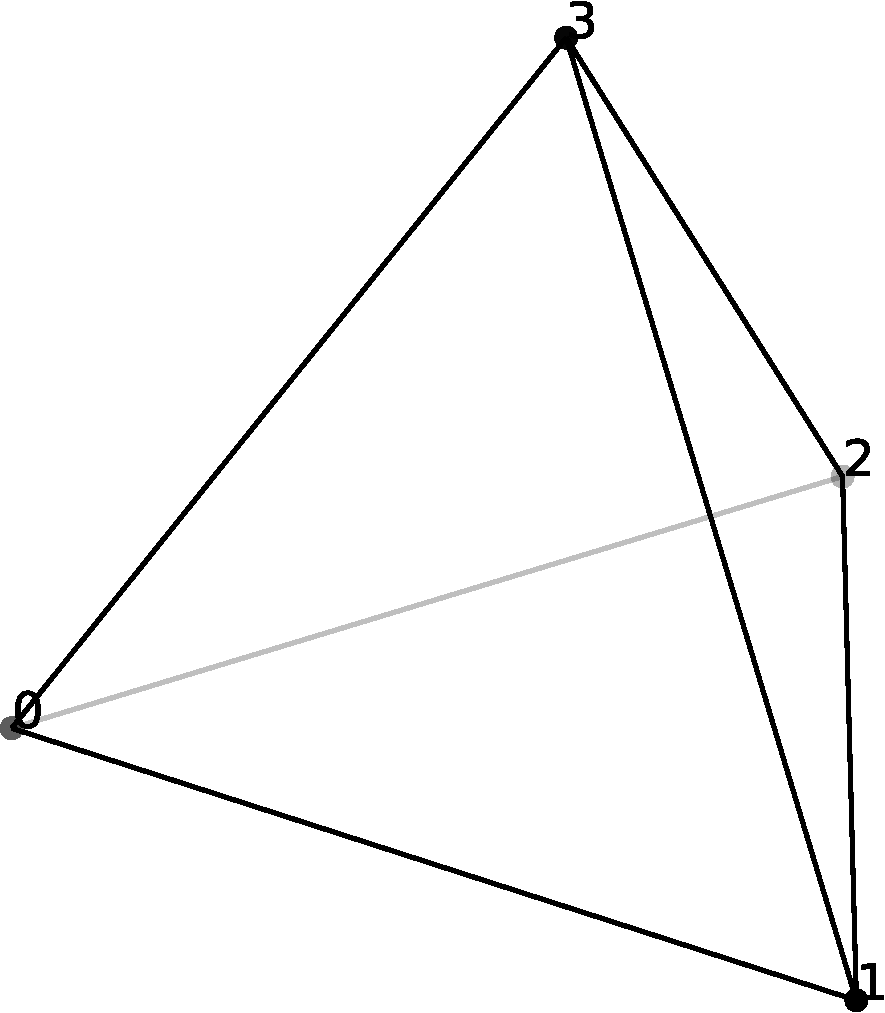
\includegraphics[scale=0.24]{figures/tet.pdf}\qquad \qquad 
%    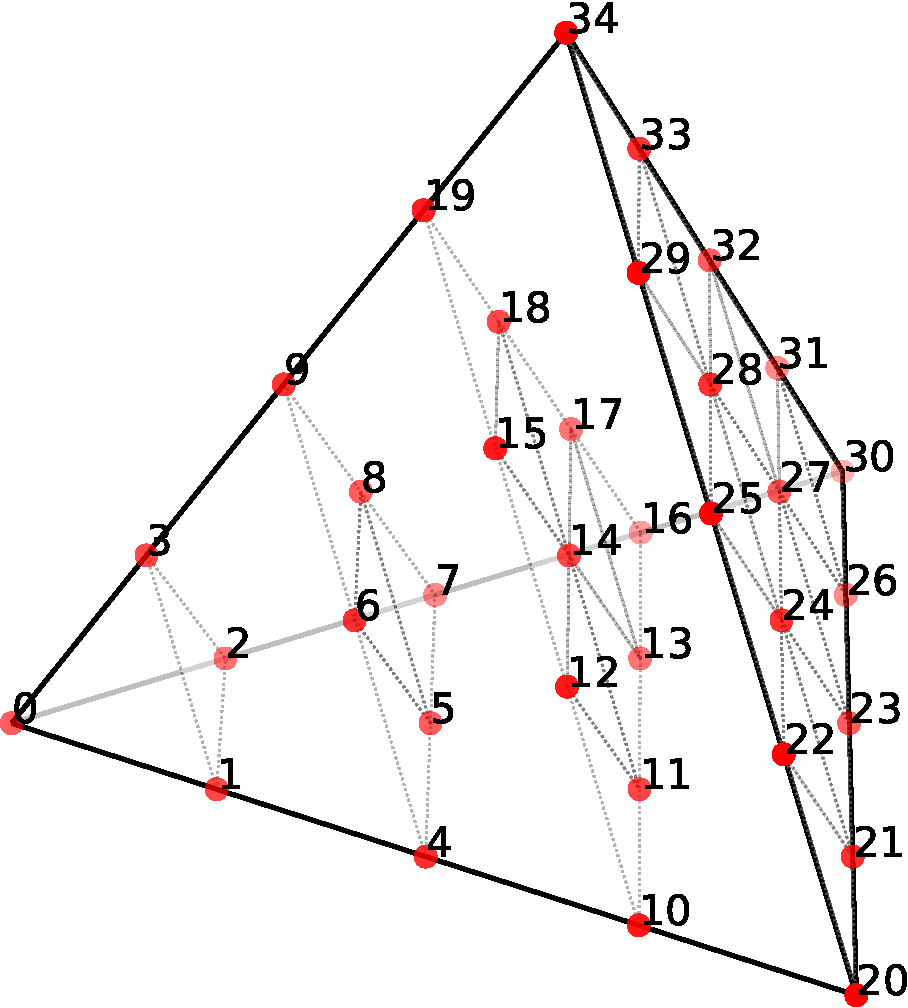
\includegraphics[scale=0.25]{figures/tetdof4.pdf}
%%\quad        \includegraphics[scale=0.25]{figures/globaltetdof4.pdf}
%    \caption{The indexing rules of tetrahedron's vertices  and interpolation points for $k=4$. Left: the local index in one element. Right: the global index in the triangulation.}
%\end{figure}


%Using the tetrahedral mesh as an illustrative example, Figure~\ref{fig:tet}
%displays the local indexing rules for the tetrahedron's vertices and the
%interpolation points when \(k=4\). 
The tetrahedron's four vertices are ordered
according to the right-hand rule, and the interpolation points adhere to the
dictionary ordering map \(R_3(\boldsymbol \alpha)\). As Lagrange
element is globally continuous, the indexing of interpolation points on the boundary $\partial T$ should be global. Namely a unique index for points on vertices, 
edges, faces should be used and a mapping from the local index to the global index is needed. 



We first set a global indexing rule for all interpolation points. We sort the index by vertices, edges, faces, and cells. For the
interpolation points that coincide with the vertices, their global index are set
as $0, 1, \ldots, \mc{NN}-1$.  When $k > 1$,  for the interpolation points that
inside edges, their global index are set as 
$$
\small
\begin{matrix}
 0\\
 1\\
 \vdots\\
 \mc{NE}-1
\end{matrix}
\begin{pmatrix}
0\cdot n_e^k &  \cdots & 1\cdot n_e^k-1\\
1\cdot n_e^k &  \cdots & 2\cdot n_e^k-1\\
 \vdots &  & \vdots \\
(\mc{NE}-1)\cdot n_e^k & \cdots & \mc{NE}\cdot n_e^k - 1\\
\end{pmatrix} +  \mc{NN}.
$$
Here recall that $n_e^k = k-1$ is the number of interior interpolation points on an edge. 
When $k>2$, for the interpolation points that inside each face, their global
index are set as  
$$
\small
\begin{matrix}
 0\\
 1\\
 \vdots\\
 \mc{NF}-1
\end{matrix}
\begin{pmatrix}
0\cdot n_f^k &  \cdots & 1\cdot n_f^k-1\\
1\cdot n_f^k &  \cdots & 2\cdot n_f^k-1\\
\vdots &  & \vdots \\
(\mc{NF}-1)\cdot n_f^k & \cdots & \mc{NF}\cdot n_f^k - 1\\
\end{pmatrix} + \mc{NN} + \mc{NE}\cdot n_e^k,
$$
where $n_f^k = (k-2)(k-1)/2$ is the number of interior interpolation points on $f$. 
When $k>3$, the global index of the interpolation points that inside
each cell can be set in a similar way. 

Then we use the two-dimensional array named \lstinline{cell2ipoint} of shape
\lstinline{(NC,ldof)} for the index map. On the $j$-th interpolation
point of the $i$-th cell, we aim to determine its unique global index and store
it in \lstinline{cell2ipoint[i,j]}.

%The combination of the simplicial lattices set \(\mathbb T^n_k\) and the
%ordering map \(R(\boldsymbol \alpha)\) readily informs the position of each
%interpolation point relative to the simplex and its sub-simplexes. If the $j$-th
%interpolation point either coincides with a vertex or is situated inside a cell,
%the global indexing rule previously discussed simplifies the assignment of
%\lstinline{cell2ipoint[i,j]}. 

For vertices and cell interpolation points, the mapping is straightforward by
the global indexing rule. Indeed \mc{cell} is the mapping of the local index of a vertex to its global index. 
However, complications arise when the
interpolation point is located within an edge or face due to non-unique representations of an edge and a face. 

We use the more complicated face interpolation points as a typical example to illustrate the situation. 
Consider, for instance, the scenario where the $j$-th interpolation point lies
within the $0$-th local face \(F_0\) of the $i$-th cell. Let \(\alpha = \)
\lstinline{m = [m0,m1,m2,m3]} be its lattice point. Given that \(F_0\) is
opposite to vertex $0$, we deduce that \(\lambda_0|_{F_0} = 0\), which implies
\lstinline{m0} is $0$. The remaining components of \lstinline{m} are non-zero,
ensuring that the point is interior to \(F_0\). 
%Using the dictionary ordering,
%we can compute its local index \(j\) as:
%\begin{align*}
%j =& \frac{(\mc{m1} + \mc{m2} + \mc{m3})(\mc{m1} + \mc{m2} + \mc{m3} + 1)(\mc{m1} + \mc{m2} + \mc{m3} + 2)}{6} \\
%&+ \frac{(\mc{m2} + \mc{m3})(\mc{m2} + \mc{m3} + 1)}{2} + \mc{m3}.
%\end{align*}

\begin{figure}[htp]
  \begin{minipage}[t]{0.48\textwidth}
  \centering
  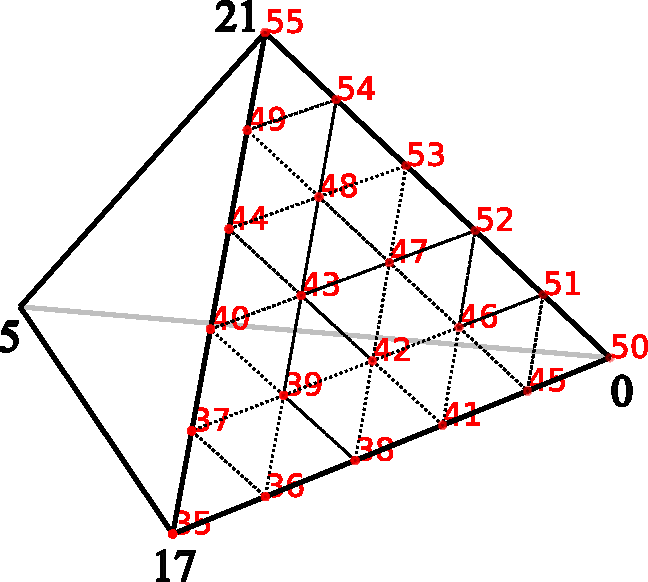
\includegraphics[width=0.82\textwidth]{figures/assigndof_ex_cell.pdf}
  \end{minipage}
  \begin{minipage}[t]{0.48\textwidth}
  \centering
  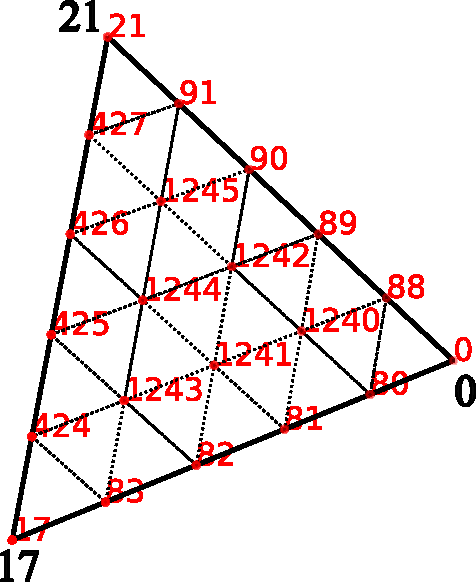
\includegraphics[width=0.6\textwidth]{figures/assigndof_ex_face.pdf}
  \end{minipage}
  \caption{Local indexing (Left) and global indexing(Right) of DoFs for a face
  of tetrahedron, where the local vertex order is \mc{[17, 0,
  21]} and global vertex order is \mc{[0, 17, 21]}. Due to the different ordering of vertices in local and global representation of the face, the ordering of the local indexing and the global indexing is different.}
  \label{fig:assigndofex}
\end{figure}

Two representations for the face with global index \lstinline{cell2face[i,0]} are subsequently acquired:
\begin{itemize}
  \item \lstinline{LFace = cell[i,SFace[0,:]]} (local representation)
  \item \lstinline{GFace = face[cell2face[i,0],:]} (global representation)
\end{itemize}
Although \lstinline{LFace} and \lstinline{GFace} comprise identical vertex
numbers, their ordering differs. For example, \mc{LFace = [5 6 10]} while \mc{GFace =[10 6 5]}. 

The array \lstinline{m = [m1,m2,m3]} has a
one-to-one correspondence with the vertices of \lstinline{LFace}. To match this
array with the vertices of \lstinline{GFace}, a reordering based on argument
sorting is performed:
\begin{lstlisting}
i0 = argsort(argsort(GFace));
i1 = argsort(LFace);
i2 = i1[i0];
m = m[i2];
\end{lstlisting}
In the example of \mc{LFace = [5 6 10]} while \mc{GFace = [10 6 5]}, the input \lstinline{m = [m1,m2,m3]} will be reordered to \lstinline{m = [m3,m2,m1]}.

From the reordered \lstinline{m = [m1,m2,m3]}, the local index \(\ell\) of the
$j$-th interpolation point on the global face \lstinline{f = cell2face[i,0]} can
be deduced:
\begin{align*}
   \ell = & \frac{(\mc{m2}-1 + \mc{m3}-1)(\mc{m2}-1 + \mc{m3}-1 + 1)}{2} + \mc{m3}-1 \\
   =& \frac{(\mc{m2} + \mc{m3} -2)(\mc{m2} + \mc{m3} - 1)}{2} + \mc{m3}-1.
\end{align*}
It's worth noting that the index of interpolation points solely within the face
needs consideration. Finally, the global index for the $j$-th
interpolation point within the $0$-th local face of the $i$-th cell is:
\[
    \mc{cell2ipoint[i j]} = \mc{NN} + n_e^k\cdot \mc{NE} + n_f^k\cdot \mc{f} + \ell.
\]

Here, we provide a specific example. Consider a 5th-degree Lagrange finite
element space on the \mc{c}-th tetrahedron in a
mesh depicted in Fig. \ref{fig:assigndofex}. The vertices of this tetrahedron
are \mc{[5,17,0,21]}, and its 0th face is denoted as \mc{f}, with vertices 
\mc{[0,17,21]}. Assuming that 
\[
    \mc{NN} + n_e^k\cdot \mc{NE} + n_f^k\cdot \mc{f} = 1240.
\]
For the 39-th local DoF on tetrahedron, 
its corresponding multi-index is \mc{[0,3,1,1]} on cell and  \mc{[3,1,1]} 
on face. Since the local face is \mc{[17,0,21]} and the global face is
\mc{[0,17,21]}, then \mc{m=[1,3,1]} and $\ell$ \mc{ =3} thus
\[
    \mc{cell2ipoint[c,39] = 1243}.
\]
Similar, for the $43$-th local DoF on tetrahedron, \mc{m = [1,2,2]} and
\mc{$\ell$=4} thus
\[
    \mc{cell2ipoint[c,43] = 1244}.
\]
Fig. \ref{fig:assigndofex} shows the correspondence between the local and the global indexing of DoFs for the cell.

In conclusion, we've elucidated the construction of global indexing for
interpolation points inside cell faces. This method can be generalized for edges
and, more broadly, for interior interpolation points of the low-dimensional
sub-simplex of an \(n\)-dimensional simplex. Please note that for scalar
Lagrange finite element spaces, the \mc{cell2ipoint} array is the mapping array
from local DoFs to global DoFs.



\subsection{Face  and edge finite element spaces}

First, we want to emphasize that the management of DoFs is to manage the
continuity of finite element space.  

The BDM and  second-kind N\'ed\'elec are vector finite element spaces, which define DoFs of
vector type by defining a vector frame on each interpolation point.
At the same time, they define their vector basis functions by combining the Lagrange
basis function and the dual frame of the DoFs.

Alternatively, we can say each DoF in BDM or second-kind N\'ed\'elec sapce corresponds to a unique interpolation point
$p$ and a unique vector $\boldsymbol e$, and each basis funcion also corresponds
to a unique Lagrange basis function which is defined on $p$ and a vector
$\hat{\boldsymbol e}$ which is the dual to  $\boldsymbol e$. 

The management of DoFs is essentially a counting problem. First of all, we need
to set global and local indexing rules for all DoFs. 
We can globally divide the DoFs into shared and unshared among simplexes. The
DoFs shared among simplexes can be further divided into on-edge and on-face
according to the dimension of the sub-simplex where the DoFs locate. First count the shared DoFs on
each edge according to the order of the edges, then count the shared DoFs on
each face according to the order of the faces, and finally count the unshared
DoFs in the cell. On each edge or face, the DoFs' order can follow the order of
the interpolation points. Note
that, for BDM and second-kind N\'ed\'elec space there are no DoFs shared on nodes. And for
3D BDM space there are no DoFs shared on edges. So the global numbering rule is
similar with the Lagrange interpolation points. 

According to the global indexing rule, we also can get a array named
\lstinline{dof2vector} with shape \lstinline{(gdof, GD)}, where \lstinline{gdof}
is the number of global DoFs and \lstinline{GD} represent geometry dimensions.
And \lstinline{dof2vector[i, :]} store the vector of the $i$-th DoF.

Next we need to set a local indexing rules and generate a array
\lstinline{cell2dof} with shape \lstinline{(NC,ldof)}, where \lstinline{ldof}
is the number of local DoFs on each cell. Note that each DoF was determined by an
interpolation point and a vector. And for each interpolation point, there is a frame
(including \lstinline{GD} vectors) on it. Given a DoF on $i$-th cell, denote the
local index  of its interpolation point as $p$, and the local index 
of its vector in the frame denote as $q$, then one can set a unique local index
number $j$ by $p$ and $q$, for example
$j = n\cdot q + p$,
where $n$ is the number of interpolation points in $i$-th cell.  Furthermore, 
we can compute the \lstinline{cell2dof[i,j]} by the global index 
\lstinline{cell2ipoint[i, p]}, the sub-simplex that the interpolation point
locate, and the global indexing rule. 

\begin{remark}\rm 
  Note that the local and global number rules  mentioned above are not unique.
  Furthermore, with the array \lstinline{cell2dof}, the implementation of these higher-order
  finite element methods mentioned in this paper is not fundamentally different
  from the conventional finite element in terms of matrix vector assembly and
  boundary condition handling. $\qed$
\end{remark}


\section{Numerical Examples}\label{sec:numerexamples}

In this section, we numerically verify the 3-dimensional BDM elements basis and the second kind
of N\'ed\'elec element basis using two test problems over the domain $\Omega =
(0, 1)^3$ partitioned into a structured tetrahedron mesh $\mathcal T_h$. All the algorithms and numerical examples are implemented based on
the FEALPy package~\cite{FEALPy}.

%\begin{figure}[htp]
%\label{fig:2}
%\centering
%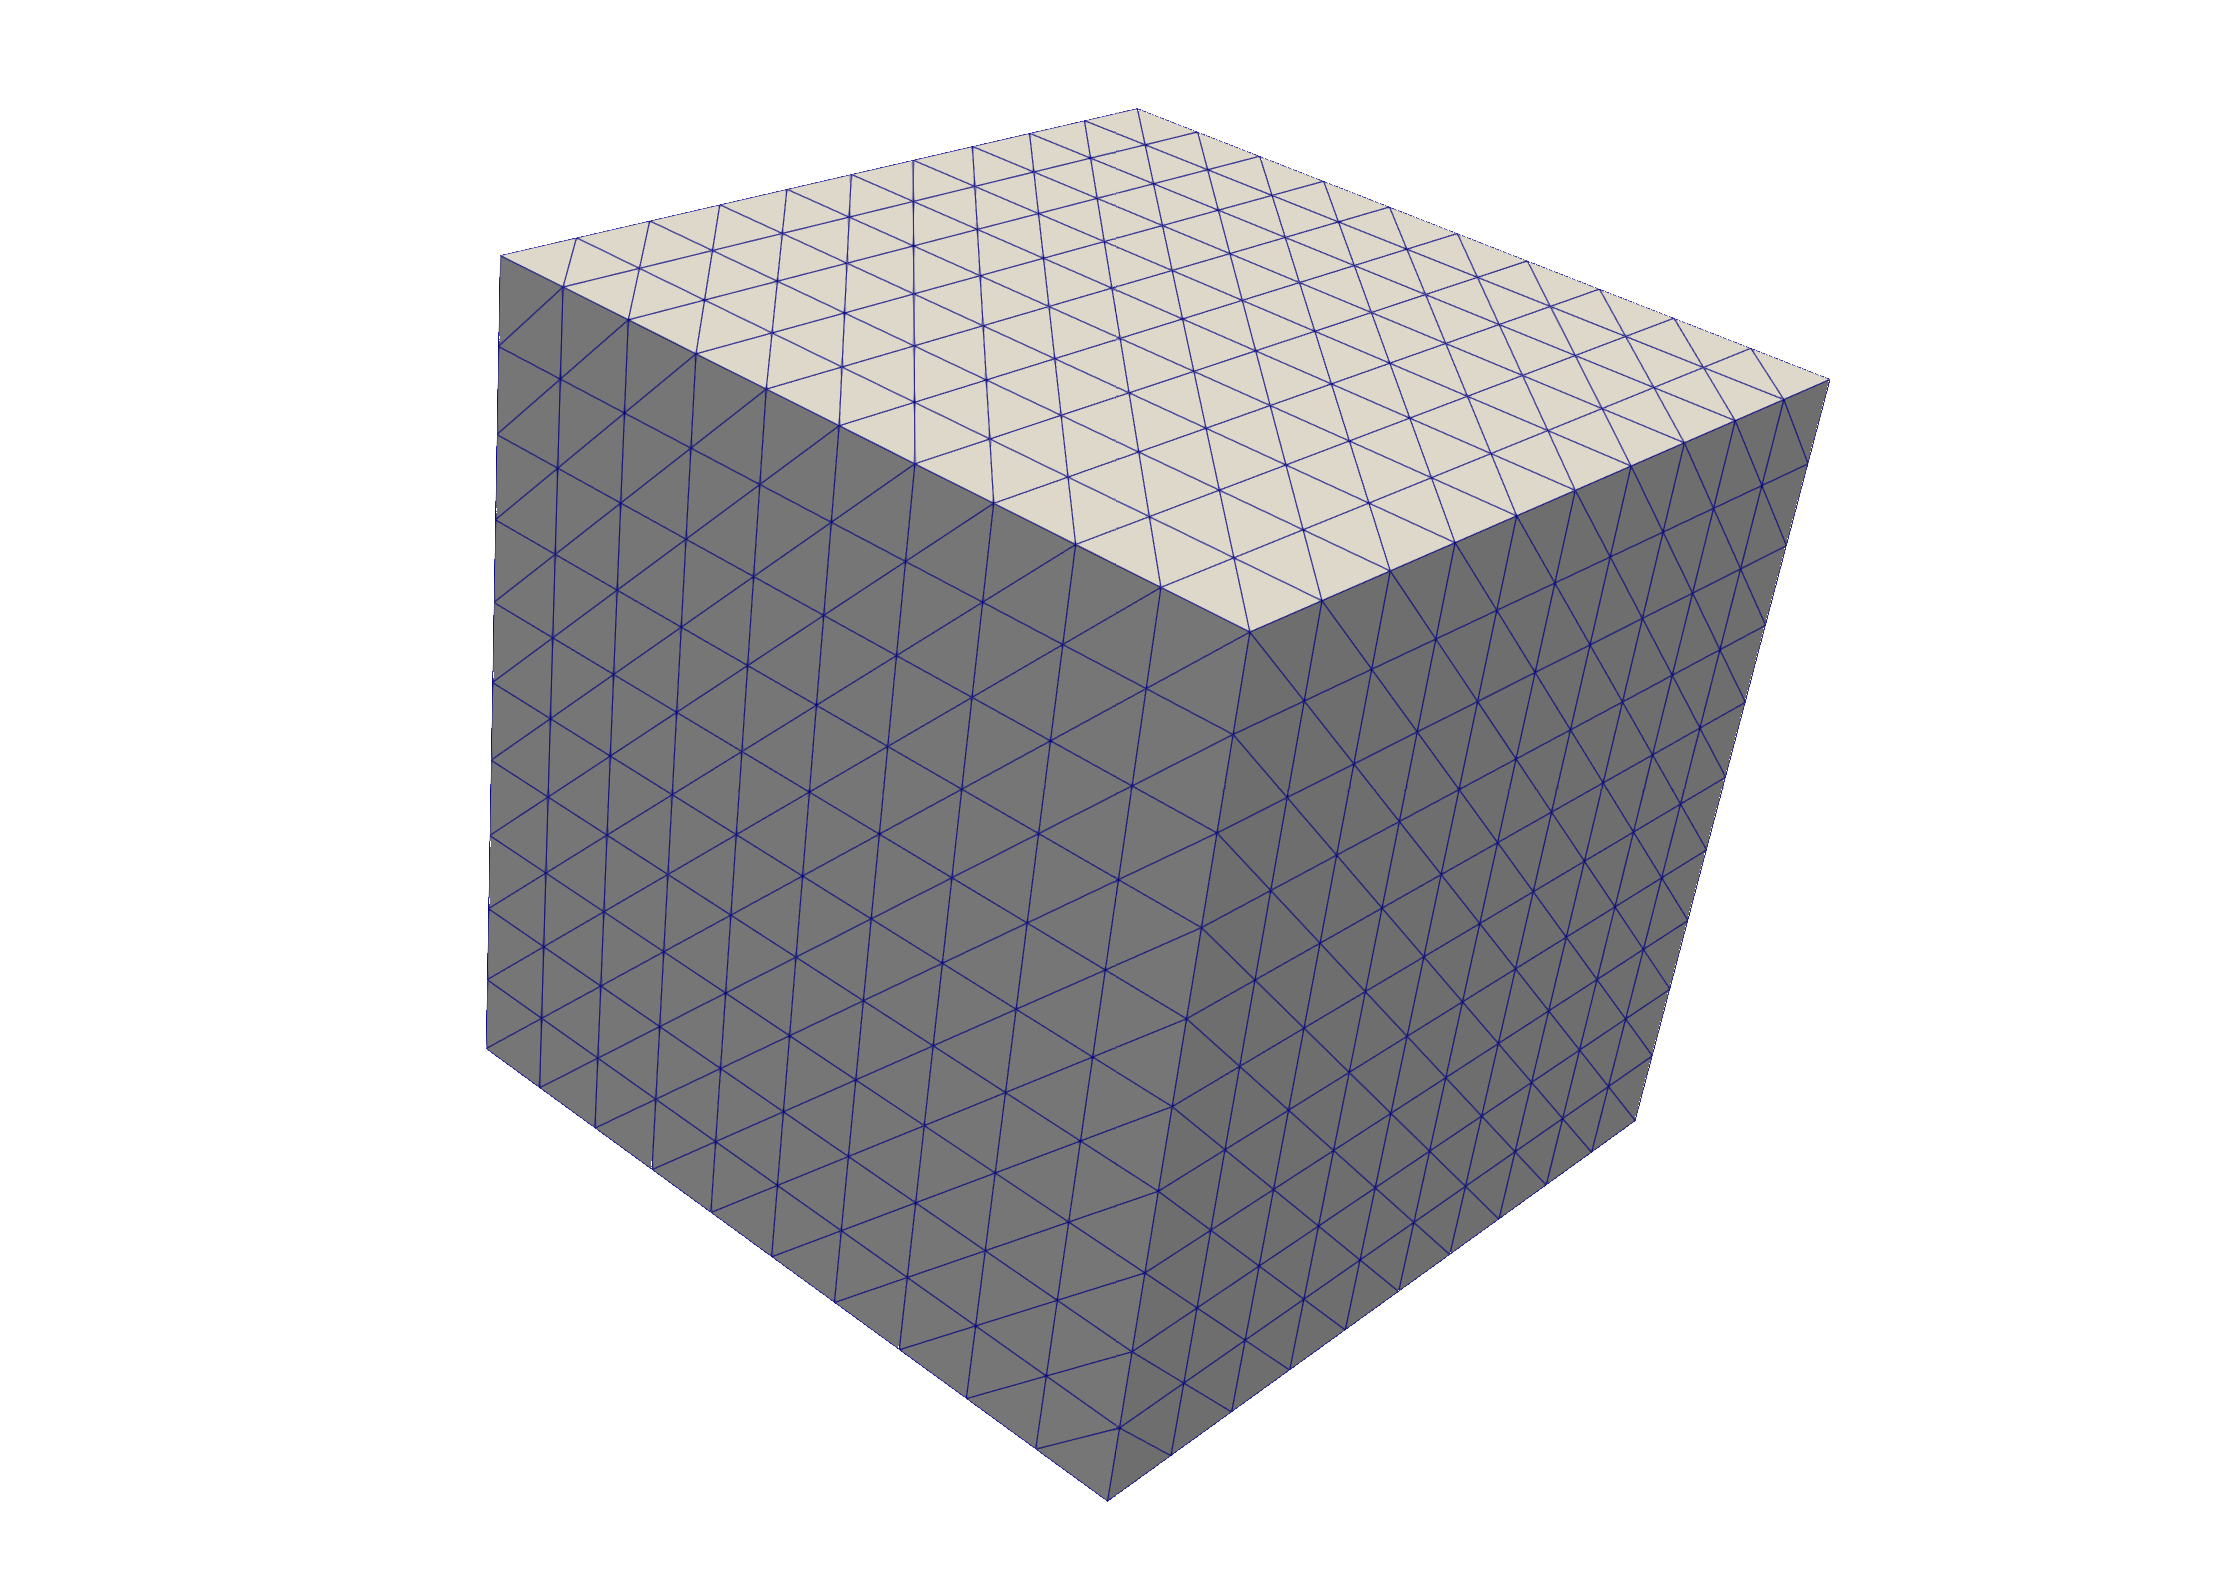
\includegraphics[width=0.6\textwidth]{figures/tet.png}
%\caption{Computational mesh corresponding to $h = 1/10$.}
%\end{figure}


\subsection{High Order Elements for Poisson Equation in the Mixed Formulation}
Consider the Poisson problem:
$$
\begin{aligned}
  \left\{
    \begin{aligned}
      \boldsymbol u + \nabla p ={}& 0 \quad \text{ in } \ \Omega,\\
      \quad \nabla \cdot \boldsymbol u ={}& f\quad \text{ in } \ \Omega,\\
      \quad \quad \ \ \  p ={}& g \quad \text{ on } \ \partial \Omega.
    \end{aligned}
  \right.
\end{aligned}
$$
The variational problem is : find 
$\boldsymbol u \in H(\mathrm{div}, \Omega)$, $p \in L^2(\Omega)$, staify:

\begin{align*}
  \int_{\Omega} \boldsymbol u \cdot \boldsymbol v \ \mathrm d\boldsymbol x -
  \int_{\Omega} p\nabla \cdot \boldsymbol v \ \mathrm d\boldsymbol x & =
  -\int_{\partial \Omega} g(\boldsymbol v \cdot \boldsymbol n) \
  \mathrm d\boldsymbol s, \quad \boldsymbol v \in H(\mathrm{div}, \Omega),\\
  -\int_{\Omega} (\nabla \cdot \boldsymbol u) q \ \mathrm d\boldsymbol x & =
  -\int_{\Omega} fq \ \mathrm d\boldsymbol x, \qquad\quad\;\;  q \in L^2(\Omega).
\end{align*}

Let $V_{h,k}^{\div}$ be the BDM space with degree $k$ on $\mathcal T_h$ and
piecewise polynomial space of degree $k-1$ on $\mathcal T_h$ by $V_{k-1}$.  
The corresponding finite element method is: find 
$\boldsymbol u_h \in V_{h,k}^{\div}, p_h \in V_{k-1}$, such that
\begin{align}
  \int_{\Omega} \boldsymbol u_h \cdot \boldsymbol v_h \ \mathrm d\boldsymbol x -
  \int_{\Omega} p\nabla \cdot \boldsymbol v_h \ \mathrm d\boldsymbol x & =
  -\int_{\partial \Omega} g(\boldsymbol v_h \cdot \boldsymbol n) \
  \mathrm d\boldsymbol s \quad  \boldsymbol v_h \in V_{h,k}^{\div},\label{exm2eq1}\\
  -\int_{\Omega} (\nabla \cdot \boldsymbol u_h) q_h \ \mathrm d\boldsymbol x &=
  -\int_{\Omega} fq_h \ \mathrm d\boldsymbol x, \qquad\quad\;  q_h \in V_{k-1}.\label{exm2eq2}
\end{align}


\begin{figure}[htp]
\centering
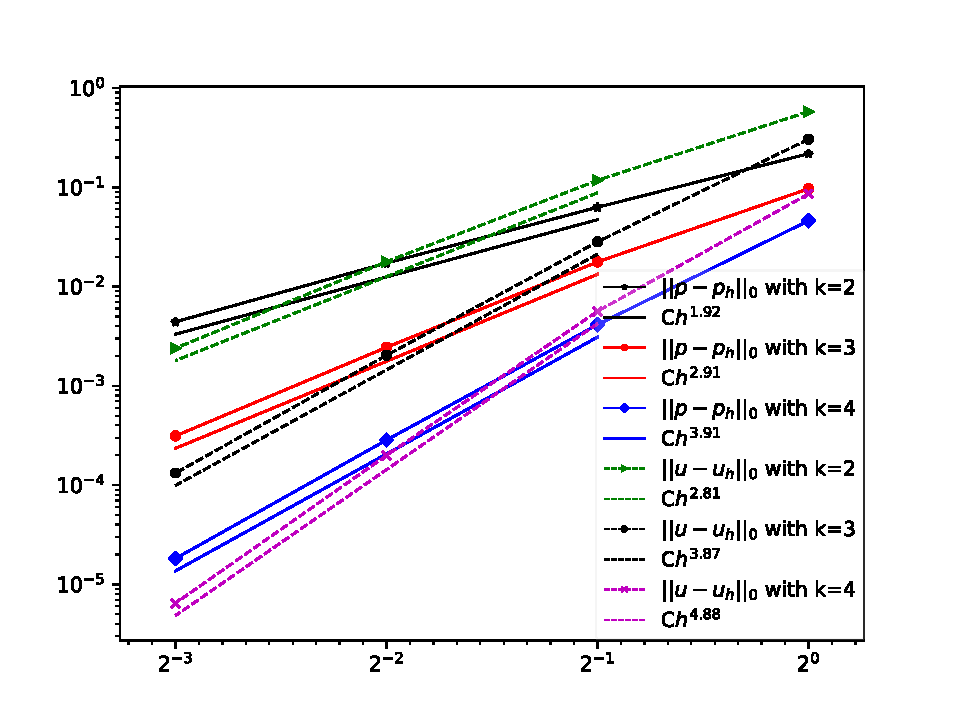
\includegraphics[width=0.6\textwidth]{figures/poisson.pdf}
\caption{Errors $\|\bs u - \bs u_h\|_0$ and $\|p - p_h\|_0$ of finite element
method \eqref{exm2eq1} and \eqref{exm2eq2} on uniformly refined mesh with $k = 2, 3, 4$.}
\label{exm2fig1}
\end{figure}

To test the convergence order of BDM space, we set
$$
\boldsymbol u = 
\begin{pmatrix}
-\pi\sin(\pi x)\cos(\pi y)\cos(\pi z)\\ 
-\pi\cos(\pi x)\sin(\pi y)\cos(\pi z)\\
-\pi\cos(\pi x)\cos(\pi y)\sin(\pi z)
\end{pmatrix},
$$
\begin{align*}
& p = \cos(\pi x)\cos(\pi y)\cos(\pi z), &  & f = 3\pi^2\cos(\pi x)\cos(\pi y)\cos(\pi z).&
\end{align*}

The numerical results are shown in Fig.~\ref{exm2fig1} and it is clear that 
$$
\|\bs u-\bs u_h\|_{0} \leq C h^{k+1}, \quad \|p - p_h\|_{0} \leq Ch^{k}.
$$

\subsection{High Order Elements for Maxwell Equations}
Consider the time harmonic problem:
$$
\begin{cases}
\nabla \times (\mu^{-1}\nabla \times \boldsymbol E) - \omega^2 \tilde \epsilon
\boldsymbol E & = \boldsymbol J \quad \text{ in } \ \ \Omega,\\
\qquad\qquad\qquad\qquad \boldsymbol n \times \boldsymbol E & = \boldsymbol 0 \quad \text{ on } \ \
\partial \Omega.
\end{cases}
$$
The variational problem is: find $\boldsymbol E \in H_0(\mathrm{curl}, \Omega),$ satisfies:
\begin{align*}
\int_{\Omega}\mu^{-1}(\nabla \times \boldsymbol E)
\cdot (\nabla \times \boldsymbol v) \ \mathrm d\boldsymbol x - 
\int_{\Omega}\omega^2 \tilde 
\epsilon \boldsymbol E \cdot \boldsymbol v\ \mathrm d\boldsymbol x
= \int_{\Omega}\boldsymbol J \cdot \boldsymbol v \ \mathrm d\boldsymbol x \quad  \forall \ \boldsymbol v \in H_0(\curl, \Omega).
\end{align*}
Let $\mathring{V}_{h,k}^{\curl} = V_{h,k}^{\curl} \cap H_0(\curl, \Omega)$, where 
$V_{h,k}^{\curl} $ is the edge element space defined in Theorem \ref{th:Nedelecelement}. The corresponding finite element method is: find 
$\boldsymbol E_h \in \mathring{V}_{h,k}^{\curl}$ s.t.
\begin{align}
\label{exm1:eq1}
\int_{\Omega}\mu^{-1}(\nabla \times \boldsymbol E_h)
\cdot (\nabla \times \boldsymbol v_h) \ \mathrm d\boldsymbol x -
\int_{\Omega}\omega^2 \tilde
\epsilon \boldsymbol E_h \cdot \boldsymbol v_h\ \mathrm d\boldsymbol x
= \int_{\Omega}\boldsymbol J \cdot \boldsymbol v_h \ \mathrm d\boldsymbol x, \quad \ 
\boldsymbol v_h \in  \mathring{V}_{h,k}^{\curl}.
\end{align} 

\begin{figure}[htp] 
\centering
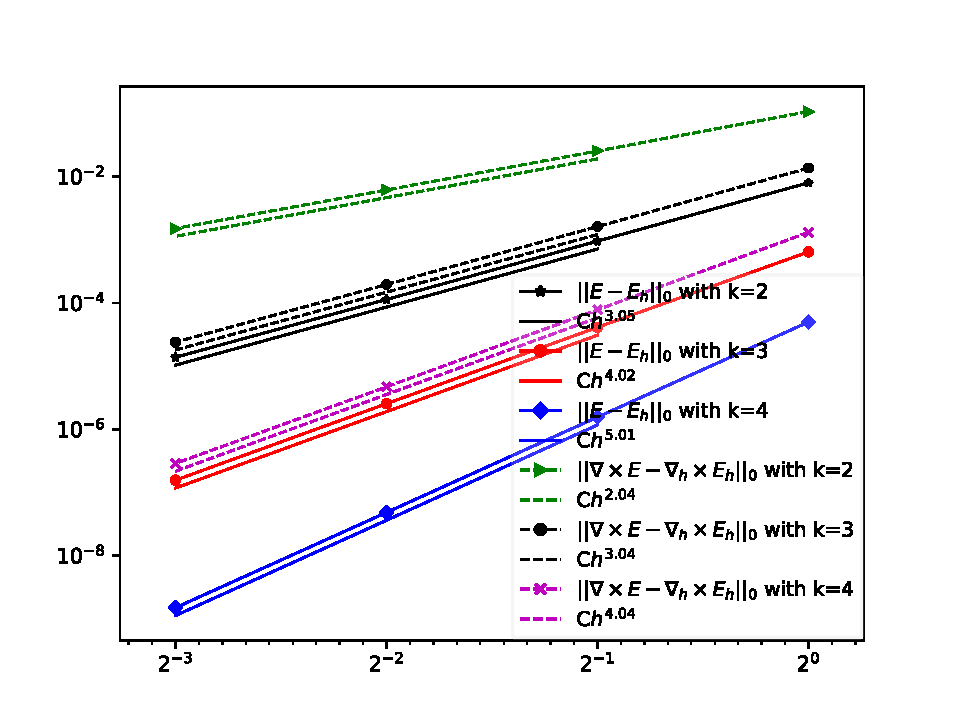
\includegraphics[width=0.6\textwidth]{figures/Maxwell.pdf}
\caption{Errors $\|\bs E - \bs E_h\|_{0}$ and 
    $\|\nabla \times(\bs E - \bs E_h)\|_{0}$ of finite element
    method \eqref{exm1:eq1} on uniformly refined mesh with $k = 2, 3, 4$.}
\label{exm1fig1}
\end{figure}

To test the convergence rate of second-kind N\'ed\'elec space, we choose 
\begin{align*}
&\omega  = \tilde \epsilon = \mu = 1, & \quad & \boldsymbol E = (f, \sin(x)f, \sin(y)f),&\\
& f = (x^2-x)(y^2-y)(z^2-z),& \quad & \boldsymbol J  = \nabla\times\nabla\times \boldsymbol E - \boldsymbol E. &
\end{align*}

The numerical results are shown in Fig.~\ref{exm1fig1} and it is clear that 
$$
\|\bs E-\bs E_h\|_{0} \leq C h^{k+1}, \quad \|\nabla\times(\bs E-\bs E_h)\|_{0} \leq C h^k.
$$


%%%% Acknowledgments %%%%%%%%
\section*{Acknowledgments}
The first and fourth authors were supported by the National Natural Science
Foundation of China (NSFC) (Grant No. 12371410, 12261131501), and the
construction of innovative provinces in Hunan Province (Grant No. 2021GK1010).
The second author was supported by NSF DMS-2012465 and DMS-2309785. The third
author was supported by the National Natural Science Foundation of China (NSFC)
(Grant No. 12171300), and the Natural Science Foundation of Shanghai (Grant No.
21ZR1480500).

%%%% Bibliography  %%%%%%%%%%
\bibliographystyle{abbrv}
\bibliography{paper}


%\begin{thebibliography}{99}
%\bibitem{Berger}M. J. Berger and P. Collela, Local adaptive mesh refinement
%for shock hydrodynamics,
%J. Comput. Phys., 82 (1989), 62-84.
%\bibitem{deBoor}C. de Boor,  Good Approximation By Splines With Variable Knots II, in Springer Lecture
% Notes Series 363, Springer-Verlag, Berlin, 1973.
%\bibitem{TanTZ} Z. J. Tan, T. Tang and Z. R. Zhang, A simple moving mesh method for one- and
%two-dimensional phase-field equations, J. Comput. Appl. Math., to appear.
%\bibitem{Toro}E. F. Toro, Riemann Solvers and Numerical Methods for Fluid Dynamics,
%Springer-Verlag Berlin Heidelbert, 1999.
%\end{thebibliography}

\end{document}
